% ---- paper/parts/00_front_intro_related.tex ----
%% Information Systems (Elsevier) -- research article.
%% Compile: python scripts/build_journal.py --paper specification_surfaces
%%
%% ROUND TWENTY-ONE.  Three reviews have been answered: a referee's report for
%% Information Systems (response_to_referee.md), a developmental review of the
%% round-nineteen manuscript (response_to_blueprint.md), and a second
%% developmental review of the round-twenty manuscript, whose twelve major
%% comments this round answers (response_to_review21.md).  REFEREE-LOG.md
%% carries the objection behind every correction.
%%
%% THE APPENDICES ARE A SEPARATE DOCUMENT, paper/supplement.tex, built by the
%% same command.  Cross-references between the two resolve through `xr'.
%%
%% EVERY NUMBER IN THIS DOCUMENT IS A MACRO defined in paper/numbers.tex,
%% which scripts/make_numbers.py generates from results/*.csv.  A number
%% therefore cannot disagree between the abstract, a table and the
%% conclusion: there is one of it.  scripts/verify_paper.py checks each
%% macro against the result file it came from.
\documentclass[preprint,12pt]{elsarticle}

%%  Latin Modern carries the bold and small-caps typewriter shapes that
%%  Computer Modern lacks -- which is what thirty font-substitution warnings
%%  in an earlier build of this round were -- and is scalable, so the PDF
%%  embeds outlines rather than bitmaps.
\usepackage{lmodern}
\usepackage{amsmath}
\usepackage{amssymb}
\usepackage{amsthm}
\usepackage{graphicx}
\usepackage{booktabs}
%%  `array' supplies the >{...} column modifier, which is what lets a narrow
%%  text column in a wide table be set ragged right instead of justified.
\usepackage{array}
\usepackage[hyphens]{url}
\urlstyle{rm}
\usepackage[protrusion=true,expansion=false]{microtype}
%%  The supplement is a separate document.  `xr' resolves a reference to one
%%  of its sections or tables to the number that document settled on, so the
%%  article can point at Section S4 without either file guessing.
\usepackage{xr}

%%  This manuscript quotes a lot of file paths in \texttt, and a typewriter
%%  path is one unbreakable word to TeX, so a paragraph that ends on one runs
%%  into the margin.  Two settings fix it without touching the prose: let a
%%  typewriter word hyphenate, and give TeX a last-resort stretch so it
%%  loosens a paragraph rather than overflowing it.  The first is what the
%%  `hyphenat' package's htt option does, written out here so that the twenty
%%  font-shape probes it performs at load time stay out of the build log --
%%  a clean log is the point of having one.
\makeatletter
\DeclareRobustCommand\texttt[1]{%
  {\ttfamily\hyphenchar\font=`\-\relax #1}}
\makeatother
\setlength{\emergencystretch}{3em}

%%  Twenty-five tables in sixty-five pages overflowed LaTeX's float queue: two
%%  of them --- the decision-curve table and the pilot's --- were deferred
%%  THIRTY pages past the text that reads them, which for a referee is the
%%  same as not having them.  The barrier keeps a table inside the section
%%  that discusses it; the fractions let a page carry more float and less
%%  compulsory text, so the barrier has somewhere to put them.
\usepackage[section]{placeins}
\renewcommand{\topfraction}{0.9}
\renewcommand{\bottomfraction}{0.8}
\renewcommand{\textfraction}{0.07}
\renewcommand{\floatpagefraction}{0.7}
\setcounter{topnumber}{3}
\setcounter{totalnumber}{5}

%% GENERATED by scripts/make_numbers.py -- do not edit.
%% Every numeric literal in the manuscript is one of these.
\newcommand{\Dabs}{+0.0899}
\newcommand{\DabsHi}{+0.1256}
\newcommand{\DabsLo}{+0.0634}
\newcommand{\Rref}{0.350}
\newcommand{\RrefKind}{bounded}
\newcommand{\VCorruptDelta}{-0.0357}
\newcommand{\VDuplicateDelta}{-0.0003}
\newcommand{\VPopCommon}{+0.1055}
\newcommand{\VPopRare}{+0.1039}
\newcommand{\VStaleDelta}{+0.0000}
\newcommand{\VTone}{+0.1835}
\newcommand{\VToneLo}{+0.1650}
\newcommand{\VTonehi}{+0.1909}
\newcommand{\VTtwoGroup}{+0.1033}
\newcommand{\VTtwoGroupHi}{+0.1106}
\newcommand{\VTtwoGroupLo}{+0.0762}
\newcommand{\VTtwoKnow}{-0.0032}
\newcommand{\VTtwoKnowHi}{+0.0013}
\newcommand{\VTtwoKnowLo}{-0.0079}
\newcommand{\agreeTolerance}{$1.1 \times 10^{-16}$}
\newcommand{\auditBJustifiedPct}{18\%}
\newcommand{\auditBStatedPct}{85\%}
\newcommand{\auditBoundHi}{48\%}
\newcommand{\auditBoundLo}{9\%}
\newcommand{\auditHalfWidthPct}{18 percentage points}
\newcommand{\auditKappa}{0.20}
\newcommand{\auditMJustifiedPct}{5\%}
\newcommand{\auditMaxWeight}{1.00}
\newcommand{\auditPrec}{0.481}
\newcommand{\auditPrecReg}{0.301}
\newcommand{\auditRangeBaselinePct}{34\%}
\newcommand{\auditRangeMetricPct}{15\%}
\newcommand{\auditRangePopulationPct}{0\%}
\newcommand{\auditRangeThresholdPct}{5\%}
\newcommand{\auditSens}{0.474}
\newcommand{\auditSensHi}{0.602}
\newcommand{\auditSensLo}{0.347}
\newcommand{\auditSensReg}{0.569}
\newcommand{\auditSpec}{0.911}
\newcommand{\auditSpecReg}{0.769}
\newcommand{\auditThetaStatedPct}{27\%}
\newcommand{\biasNoisyBefore}{-0.0353}
\newcommand{\biasOracleMax}{0.0405}
\newcommand{\cardF}{3{,}019}
\newcommand{\casePrevalence}{0.372}
\newcommand{\corruptLevel}{15\%}
\newcommand{\coverageNaiveMedian}{90.5\%}
\newcommand{\coverageNaiveMin}{5.5\%}
\newcommand{\coverageNestedBasicMedian}{92.0\%}
\newcommand{\coverageNestedBasicMin}{7.0\%}
\newcommand{\coverageNestedBcMedian}{91.5\%}
\newcommand{\coverageNestedMedian}{94.2\%}
\newcommand{\coverageNestedMin}{3.5\%}
\newcommand{\coverageNoisyAfter}{7.0\%}
\newcommand{\coverageNoisyBefore}{7.0\%}
\newcommand{\crossTargetAgreement}{45\%}
\newcommand{\doiBPICfourteen}{\url{https://doi.org/10.4121/uuid:c3e5d162-0cfd-4bb0-bd82-af5268819c35}}
\newcommand{\doiBPICthirteen}{\url{https://doi.org/10.4121/uuid:500573e6-accc-4b0c-9576-aa5468b10cee}}
\newcommand{\exCells}{480}
\newcommand{\exMisreportPct}{24.9\%}
\newcommand{\exRmax}{0.947}
\newcommand{\exRmin}{0.200}
\newcommand{\exRows}{30{,}162}
\newcommand{\exSbaselinePct}{25.9\%}
\newcommand{\exSmetricPct}{25.9\%}
\newcommand{\exSpopulationPct}{7.2\%}
\newcommand{\exampleLines}{121}
\newcommand{\flipLearnerPct}{31.3\%}
\newcommand{\flipMetricPct}{19.7\%}
\newcommand{\flipQualityPct}{20.4\%}
\newcommand{\flipRungPct}{22.2\%}
\newcommand{\flipSplitPct}{33.5\%}
\newcommand{\fvVersion}{0.2.0}
\newcommand{\gridHi}{0.80}
\newcommand{\gridLo}{0.05}
\newcommand{\kmBaseAuc}{0.648}
\newcommand{\kmOrphanPopulated}{100\%}
\newcommand{\lambdaHalf}{0.64}
\newcommand{\lambdaHalfPct}{64\%}
\newcommand{\limitNoisyAfter}{+0.1135}
\newcommand{\limitNoisyBefore}{+0.1135}
\newcommand{\maxCardBZero}{200}
\newcommand{\maxTMedian}{4.03}
\newcommand{\maxTMedianRatio}{2.06}
\newcommand{\meanNoisyEstimate}{+0.0781}
\newcommand{\minCardF}{50}
\newcommand{\minGPresent}{50\%}
\newcommand{\minPerStratum}{25}
\newcommand{\minReuseF}{two}
\newcommand{\minTrainCoverage}{50\%}
\newcommand{\misreportMaxPct}{57.7\%}
\newcommand{\misreportMedianPct}{35.3\%}
\newcommand{\misreportMinPct}{5.6\%}
\newcommand{\nAgreeDisagree}{0}
\newcommand{\nAgreeQuantities}{266}
\newcommand{\nAuditApplicable}{3}
\newcommand{\nAuditEffective}{29.6}
\newcommand{\nAuditEligible}{54.9}
\newcommand{\nAuditFrame}{600}
\newcommand{\nAuditFullText}{369}
\newcommand{\nAuditNoFullText}{231}
\newcommand{\nAuditOutSampled}{120}
\newcommand{\nAuditRequired}{196}
\newcommand{\nAuditSampled}{600}
\newcommand{\nAuditScreenedIn}{54}
\newcommand{\nAuditScreenedOut}{315}
\newcommand{\nAuditStrata}{77}
\newcommand{\nAuditTarget}{2{,}400}
\newcommand{\nAxes}{nine}
\newcommand{\nBandResolvedRaw}{2{,}046}
\newcommand{\nBandResolvedRecentred}{2{,}163}
\newcommand{\nCaseTest}{13{,}637}
\newcommand{\nCaseTrain}{31{,}818}
\newcommand{\nClosedBefore}{5}
\newcommand{\nCohort}{45{,}455}
\newcommand{\nCohortCorpus}{46{,}606}
\newcommand{\nCondBeneficial}{11}
\newcommand{\nCondHarmful}{1}
\newcommand{\nConditions}{8}
\newcommand{\nConfirmReject}{5}
\newcommand{\nCorpusLogs}{21}
\newcommand{\nDomains}{6}
\newcommand{\nDrawRows}{1{,}791{,}720}
\newcommand{\nFieller}{10{,}584}
\newcommand{\nFiellerUnbounded}{5{,}282}
\newcommand{\nFolds}{five}
\newcommand{\nGrid}{31}
\newcommand{\nHarmfulPointwise}{0}
\newcommand{\nHarmfulSimultaneous}{0}
\newcommand{\nLearners}{4}
\newcommand{\nLogs}{13}
\newcommand{\nLogsBothTargets}{6}
\newcommand{\nMeanOptimal}{19}
\newcommand{\nMetrics}{36}
\newcommand{\nMisreportOverQuarter}{13}
\newcommand{\nMisreportOverTen}{18}
\newcommand{\nOneNumberOptimal}{9}
\newcommand{\nOrphans}{94{,}250}
\newcommand{\nPairs}{19}
\newcommand{\nPairsBanded}{19}
\newcommand{\nPenaltyDecades}{five}
\newcommand{\nPropN}{1{,}800}
\newcommand{\nPropP}{200}
\newcommand{\nQuality}{10}
\newcommand{\nResultEstates}{18}
\newcommand{\nResultPairs}{12}
\newcommand{\nScaleReps}{\textbf{??}}
\newcommand{\nSeeds}{three}
\newcommand{\nSignChanging}{4}
\newcommand{\nSignVaries}{18}
\newcommand{\nSimReps}{200}
\newcommand{\nSimSparse}{200}
\newcommand{\nSizeGrid}{six}
\newcommand{\nSplits}{6}
\newcommand{\nSurfaceRows}{262{,}656}
\newcommand{\nTests}{108}
\newcommand{\nTrainOnly}{122}
\newcommand{\nTrainOnlyPassed}{122}
\newcommand{\nUniformlyBeneficial}{1}
\newcommand{\nUnresolvedPairs}{2}
\newcommand{\nWorkedBefore}{41{,}413}
\newcommand{\nWorlds}{six}
\newcommand{\noisyGapLarge}{\textbf{??}}
\newcommand{\noisyGapLoose}{\textbf{??}}
\newcommand{\noisyGapSmall}{\textbf{??}}
\newcommand{\noisyGapTight}{\textbf{??}}
\newcommand{\pThreeRawA}{0.421}
\newcommand{\pThreeRawB}{0.284}
\newcommand{\pThreeSqrtA}{0.232}
\newcommand{\pThreeSqrtB}{0.390}
\newcommand{\prevHi}{0.95}
\newcommand{\prevLo}{0.05}
\newcommand{\propOneApGap}{0.988}
\newcommand{\propOneAucGap}{exactly zero}
\newcommand{\propOneSweepAp}{0.998}
\newcommand{\propOneSweepAuc}{$4.4 \times 10^{-15}$}
\newcommand{\propTwoCancelShift}{machine precision}
\newcommand{\propTwoNonRankShift}{11.696}
\newcommand{\propTwoRankShift}{exactly zero}
\newcommand{\qClean}{+0.1673}
\newcommand{\qCommonHalf}{+0.1055}
\newcommand{\qCorruptThirty}{-0.0699}
\newcommand{\qDuplicateAll}{-0.0038}
\newcommand{\qLagHalfDelta}{-0.0031}
\newcommand{\qLagHalfPopulated}{94.1\%}
\newcommand{\qRandomHalf}{+0.0951}
\newcommand{\qRareHalf}{+0.1039}
\newcommand{\qStaleDelta}{+0.0000}
\newcommand{\qStaleKeepsDelta}{+0.0000}
\newcommand{\ratioBase}{2.3}
\newcommand{\ratioCheap}{9.0}
\newcommand{\ratioDear}{0.7}
\newcommand{\regretMajority}{0.0297}
\newcommand{\regretMajorityAdj}{0.0197}
\newcommand{\regretMajorityGainAdjPct}{18.3\%}
\newcommand{\regretMajorityGainPct}{21.9\%}
\newcommand{\regretMeanRule}{0.0242}
\newcommand{\regretOneNumber}{0.0380}
\newcommand{\regretOneNumberAdj}{0.0241}
\newcommand{\regretOneNumberExcessPct}{57.2\%}
\newcommand{\regretOracle}{0.0242}
\newcommand{\regretUniformRule}{0.0489}
\newcommand{\releaseTag}{v19.0}
\newcommand{\resultWitnessMax}{5}
\newcommand{\resultWitnessMin}{0}
\newcommand{\rhoMedian}{0.200}
\newcommand{\shiftMedian}{-0.0001}
\newcommand{\shiftNegativePct}{56\%}
\newcommand{\simNoiseRate}{20\%}
\newcommand{\simPrevalence}{0.02}
\newcommand{\sizeHi}{\textbf{??}}
\newcommand{\sizeLo}{\textbf{??}}
\newcommand{\sobolInteractionPct}{30.0\%}
\newcommand{\sobolLearnerPct}{2.6\%}
\newcommand{\sobolMaxAxis}{the metric}
\newcommand{\sobolMaxPct}{10.1\%}
\newcommand{\sobolMetricPct}{10.1\%}
\newcommand{\sobolQualityPct}{2.7\%}
\newcommand{\sobolRungPct}{1.9\%}
\newcommand{\sobolSplitPct}{9.4\%}
\newcommand{\sobolTargetPct}{2.1\%}
\newcommand{\sobolTopAxis}{the split}
\newcommand{\sobolTopPair}{BPIC19/duration}
\newcommand{\sobolTopPct}{50.7\%}
\newcommand{\sparseGapLarge}{\textbf{??}}
\newcommand{\sparseGapSmall}{\textbf{??}}
\newcommand{\spreadHeadline}{0.091 AUC at the median pair and 0.298 at the widest}
\newcommand{\spreadMax}{0.298}
\newcommand{\spreadMedian}{0.091}
\newcommand{\targetAgreement}{51\%}
\newcommand{\targetAgreementHi}{66\%}
\newcommand{\targetAgreementLo}{43\%}
\newcommand{\thetaBase}{0.30}
\newcommand{\thetaCheap}{0.10}
\newcommand{\thetaDear}{0.60}
\newcommand{\unseenMax}{87\%}
\newcommand{\unseenMin}{0\%}
\newcommand{\widthNoisyBefore}{0.0367}
\newcommand{\zenodoDOI}{the archived release cited in the data-availability statement (DOI reserved, inserted at proof)}


\externaldocument{supplement}

\newtheorem{proposition}{Proposition}
\newtheorem{lemma}{Lemma}
\newtheorem{corollary}{Corollary}
\newtheorem{definition}{Definition}
\newtheorem{remark}{Remark}
\theoremstyle{definition}
\newtheorem{assumption}{Assumption}

\journal{Information Systems}

\begin{document}

\begin{frontmatter}

\title{Specification Surfaces for Incremental Predictive Performance:
Estimation, Uncertainty, and Multi-Log Evaluation}

\author[ind]{Sudhir Dixit}
\ead{sudhir.dixit1@gmail.com}
\address[ind]{Independent Researcher}

\begin{abstract}
What a recorded field is worth to a prediction is reported as one number, but
that number is a functional of rarely stated choices: baseline, pipeline,
target, split, decision time, register quality, metric and operating point. We
define incremental predictive performance as a \emph{specification surface}
$V_s(f)$ over a declared design space under a declared measure, and give four
objects for reporting one: an exact functional-ANOVA decomposition of its
variance; simultaneous max-$t$ bands over the \emph{whole} surface a claim
ranges over, from a pipeline-refitting moving-block bootstrap; \emph{resolution
regions} with a robustness index; and \emph{specification regret}. On \nPairs\ log--target
pairs from \nLogs\ public event logs, over an audited
\nDeclaredAdmissibleScalar-cell space, the baseline alone moves the increment
by \spreadMedian\ AUC at the median pair, and a one-number report misstates
the sign of \misreportPooledResolvedPct\ of resolved cells ---
\misreportPooledItsmPct\ on the \nItsmPairs\ maintained registers. Of the
\nPairsResolvingAny\ pairs resolving any sign, \nPairsResolveBothSigns\ resolve
both. On \nModelsDcaExcluded\ of \nModelsDca\ models a threshold is not a
cost ratio at all. In a case study on \nCohort\ bank incidents, a register's
value turns on the decision time and its sign on the target.
\end{abstract}

%%  Six keywords: the Elsevier template caps them at six and an earlier
%%  version listed seven.
\begin{keyword}
specification surface \sep incremental predictive performance \sep
predictive process monitoring \sep simultaneous inference \sep
sensitivity analysis \sep configuration management database
\end{keyword}

\end{frontmatter}

%%  Highlights.  Elsevier collects these in a separate file; they are printed
%%  here as well so that a reviewer holding only the PDF can see them.  The
%%  text is generated into numbers.tex from submission/highlights.txt by
%%  scripts/make_numbers.py, and scripts/check_highlights.py enforces the
%%  three-to-five count and the eighty-five-character limit, so the two
%%  copies cannot drift and neither can be over length.
\section*{Highlights}
\begin{itemize}\itemsep0pt
\highlightsList{}
\end{itemize}

\section{Introduction}
\label{sec:intro}

A claim that a recorded field is worth something is a comparison. Its second
arm --- performance \emph{without} the field --- is a choice the analyst
makes, and so are the learner that makes the comparison, the encoding it uses,
the outcome it predicts, the way the data are split in time, whether the field
is available at the moment the decision is taken, how completely the register
behind the field is populated, the metric the difference is read in, and the
operating point at which that metric is evaluated. Each is routinely left
implicit, and the result is reported as one number.

This paper's position is not that such a number depends on those choices ---
that is known, and Section~\ref{sec:related} says by whom --- but that the
dependence is large enough, on real decisions, to change the sign of the
answer; that the right object to report is therefore a surface over a
\emph{declared} design space rather than a point; and that a surface admits
estimation and inference of its own.

\paragraph{The estimand}
Write a specification $s$ for a complete assignment to every design axis, and
\begin{equation}
V_s(f) \;=\; m_\theta\!\left(A_s(D_{\mathrm{train}}, B \cup \{f_q\}),\,
D_{\mathrm{test}}\right)
\;-\;
m_\theta\!\left(A_s(D_{\mathrm{train}}, B),\, D_{\mathrm{test}}\right),
\label{eq:estimand}
\end{equation}
where $A_s$ is the fitting procedure (learner, encoding, hyperparameters,
calibration), $B$ the baseline feature set, $f_q$ the field under a register
quality mechanism $q$, $m$ the metric and $\theta$ the operating point, and
where $D_{\mathrm{train}}, D_{\mathrm{test}}$ are fixed by the split rule and
the cohort. The \emph{specification surface} is the map
$s \mapsto V_s(f)$ over a design space $\mathcal{S}$ that the analyst declares
and the reader can enumerate; Figure~\ref{fig:speccurve} draws one.

We say \emph{incremental predictive performance} and not \emph{value}:
\eqref{eq:estimand} measures how much better a model predicts, not what the
field costs to acquire or maintain, whether acting on the prediction changes
the outcome, or what an organisation would pay for either.
Section~\ref{sec:dca} converts the increment into net benefit at a declared
exchange rate, which is as close to economic value as this evidence gets.

\begin{figure}[!t]
\centering
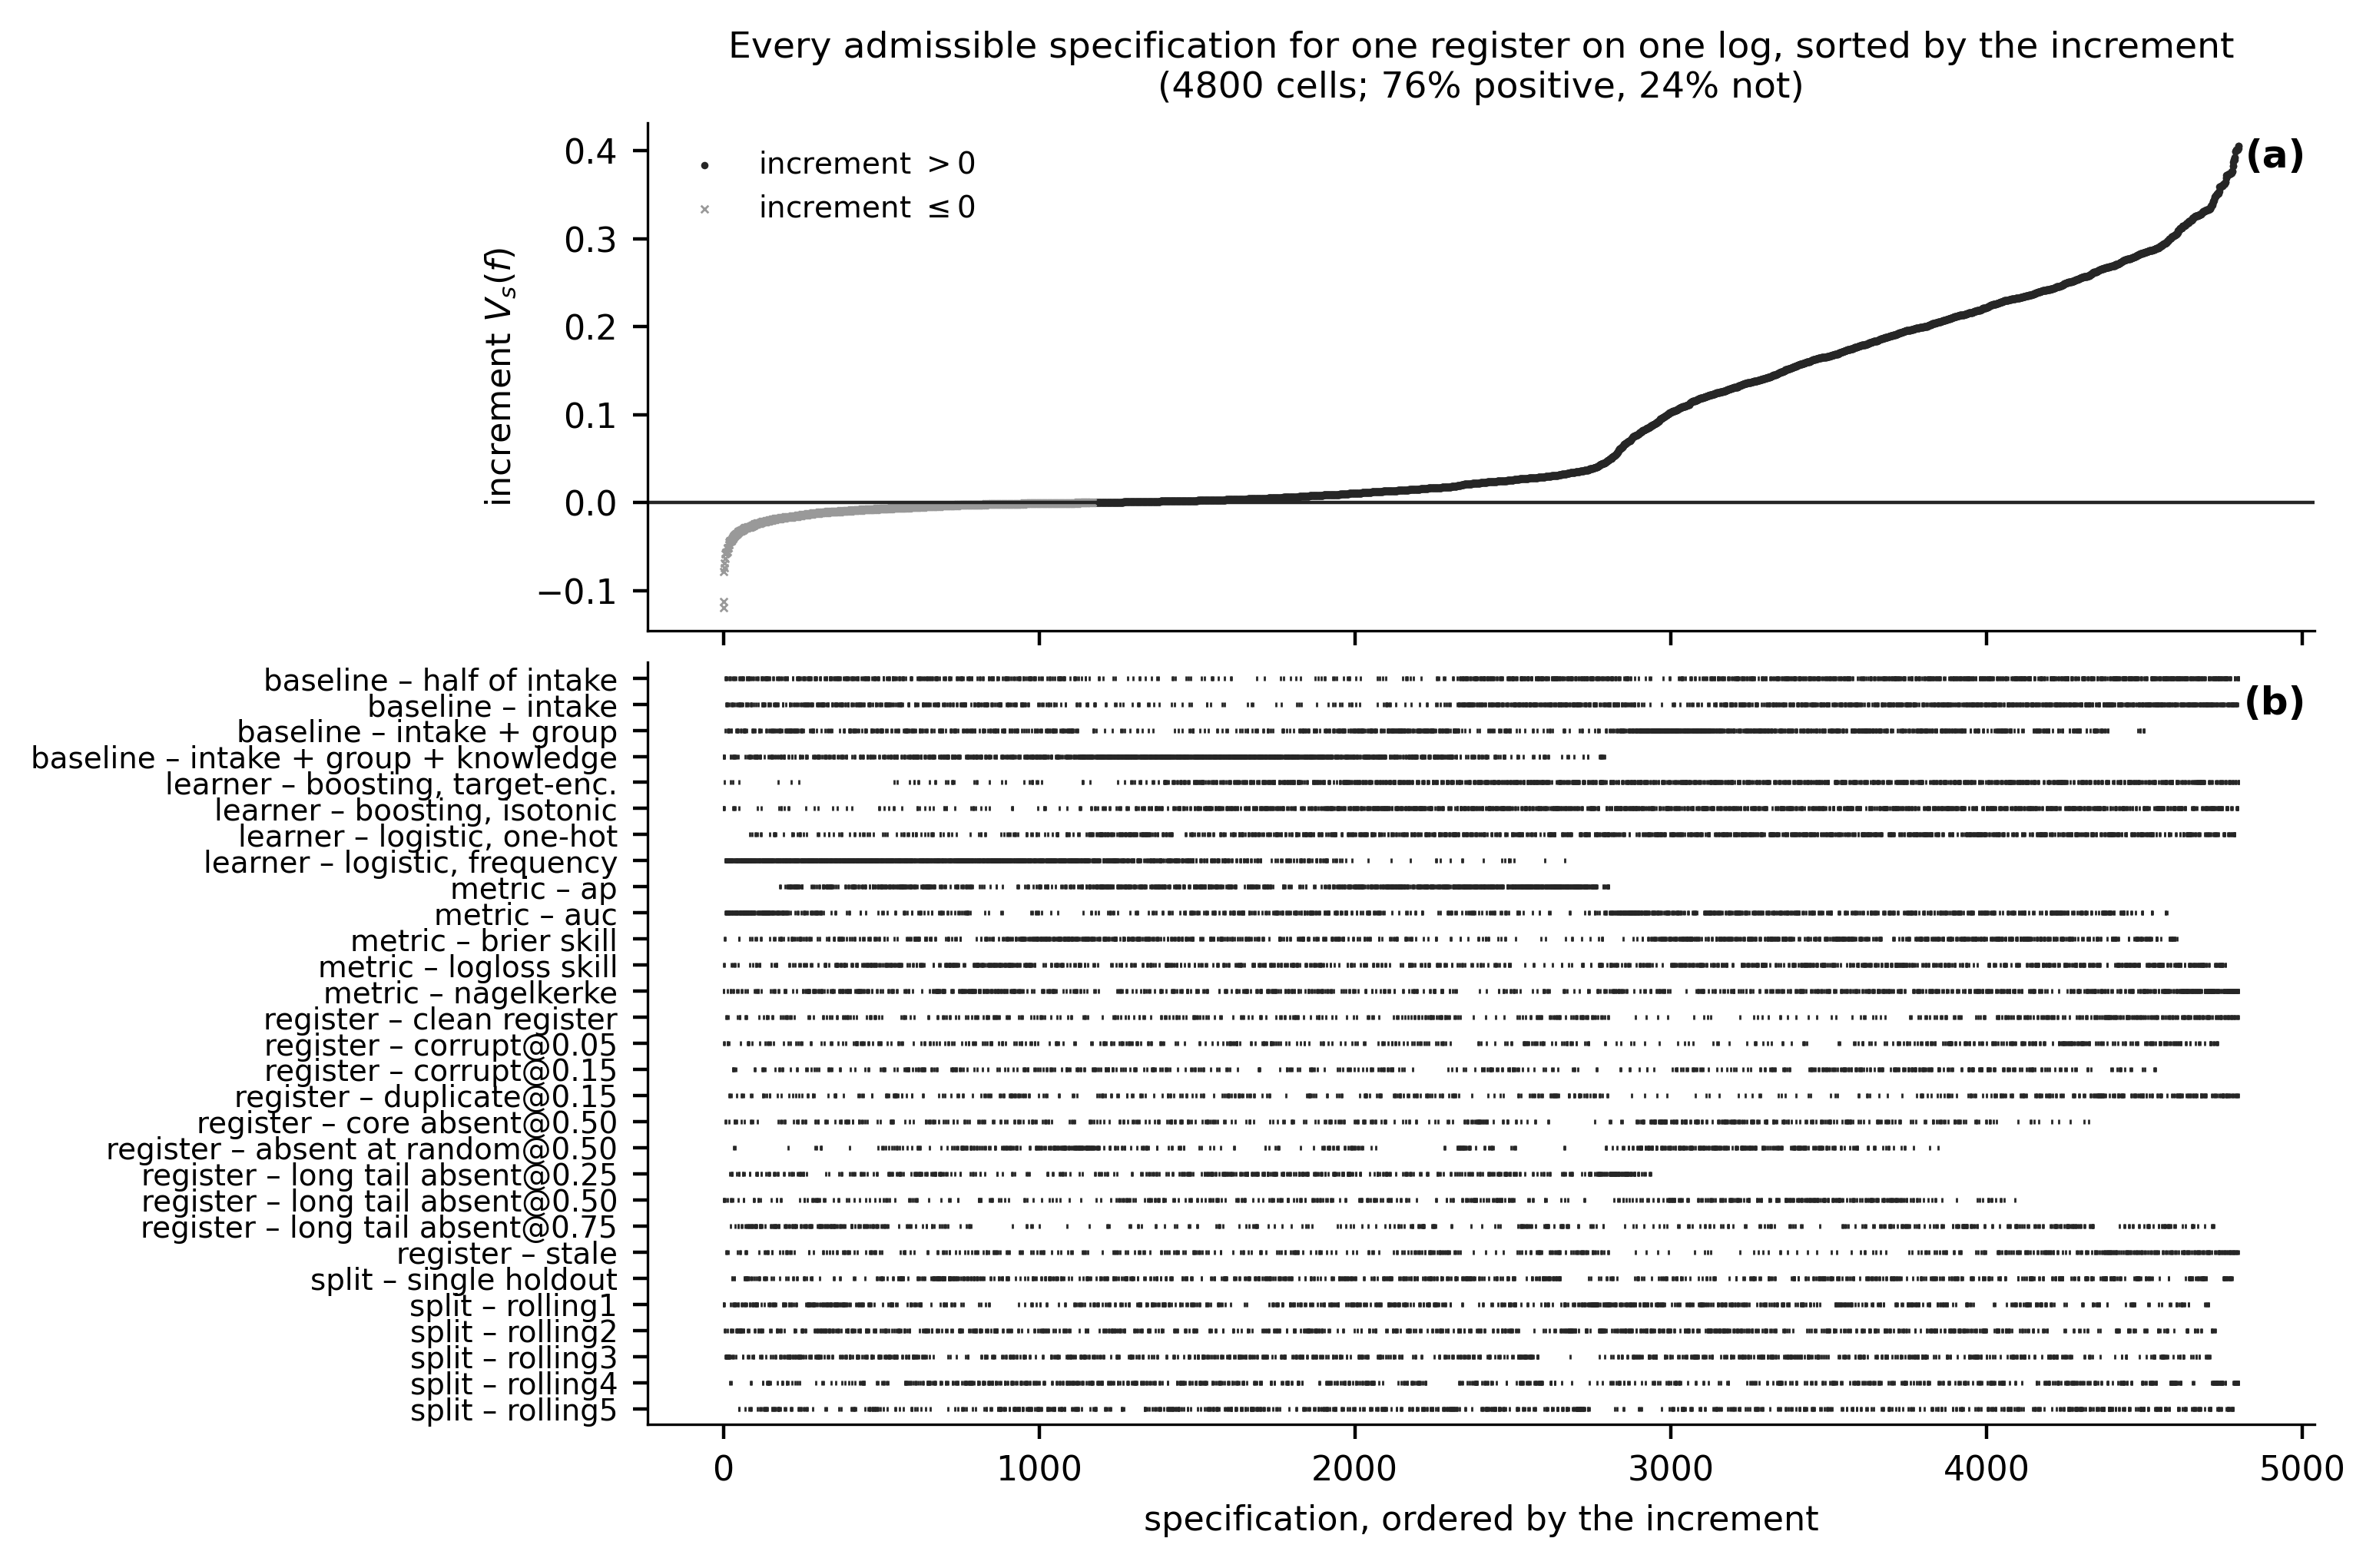
\includegraphics[width=\linewidth]{figS1_speccurve.png}
\caption{The specification curve for the configuration item on BPIC14, at the
registered handover target. \textbf{(a)} Each point is one admissible
specification --- a complete assignment to the pipeline, the baseline rung,
the register-quality condition, the split and the metric --- sorted by the
increment. \textbf{(b)} Which level of which axis each specification occupies.
The intercept-only rung is excluded. Every point is a point estimate; the
simultaneous bands that decide the region labels are in
Table~\ref{tab:calbands}. \textbf{The five scalar instruments are plotted on
one axis and their increments are not on a common scale}
(Section~\ref{sec:regretdef}); what the panel supports is the \emph{sign}
statement, which is unit-free, and not a comparison of magnitudes across
instruments. The panel shows the increment rather than the reduction, so a
cell where the register is worth almost nothing looks the same as one where
the free field absorbs almost everything.}
\label{fig:speccurve}
\end{figure}

\paragraph{Contributions}
Multiverse and specification-curve analysis, functional-ANOVA and Sobol
indices, the moving-block bootstrap, max-$t$ and multiplier bootstraps,
decision curve analysis, calibration assessment, and feature and data
valuation are all established, and none of them is invented here;
Section~\ref{sec:related} attributes each and states the gap they leave. What
follows is what this paper adds.

\begin{enumerate}
\item \textbf{A new formalisation: the specification surface and a complete
estimand.} Section~\ref{sec:surface} defines $\mathcal{S}$, $V_s$, and the
relative reduction $R$, states the conditions under which $R$ is a quantity at
all, and proves two results. $R$ is \emph{not identified} by the data, the
feature and the baselines: there is no function carrying the reduction under
one metric to the reduction under another (Proposition~\ref{prop:nonid}). And,
relative to a \emph{declared family} of recalibrations, $R$ survives every
member of that family exactly when each member acts \emph{affinely} on the
instrument (Proposition~\ref{prop:rank}) --- which within the affine family is
strictly weaker than rank-basedness, and outside it is not
(Section~\ref{sec:weaker}). The proposition also converts
a search into a proof: one violating triple settles an instrument for the
family it was found in.

\item \textbf{New reporting objects: two adaptations and two new.}
Section~\ref{sec:inference} supplies the estimation and inference layer. Four
constructions are taken from the literature and two of them are
\emph{adapted}: (i) an exact, orthogonal functional-ANOVA decomposition of
$\operatorname{Var}_s[V_s(f)]$ into first-order and total indices per axis,
taken here under a \emph{declared measure} over specifications rather than
under whichever cells happened to be enumerated; (ii) a moving-block bootstrap
that resamples the training half, \emph{refits the entire pipeline}, and
evaluates on a resampled test half, so the interval contains training-sample,
model-selection, encoder and calibrator variability; (iii) simultaneous
max-$t$ bands whose family, for a surface-level claim, is the \emph{whole
surface} that claim ranges over and not a cell of it, with the critical value
estimated by a multiplier bootstrap so that its precision is not limited by
the refitting budget; and (iv) Fieller intervals for $R$, which report an
unbounded or exclusive confidence set when the denominator is weak instead of
a bounded interval that is not one.

Two further objects are new as far as we are aware. A cell is
\emph{beneficial}, \emph{harmful} or \emph{unresolved} under the simultaneous
band, a surface carries one of six \emph{resolution region} labels, and the
robustness index $\rho \in [-1,1]$ summarises it; $\rho = 1$ is the only state
in which one positive number is a safe summary. And \emph{specification
regret} measures what one-number reporting costs --- the share of admissible
specifications whose sign disagrees with the reported cell, and the
performance forgone or destroyed by acting on it, computed \emph{inside one
instrument at a time}. Lemma~\ref{prop:optimal} identifies the
decision-optimal collapse, the weighted mean increment, and
Section~\ref{sec:rules} measures four rules against it \emph{out of sample},
on held-out specifications, held-out time and held-out logs.

\item \textbf{New empirical evidence: a registered multi-log benchmark.} The
surface is computed through one frozen pipeline on \emph{every} log--target
pair a pre-registered protocol admits --- \nPairs\ of them, not only the ones
where the answer resolves --- over an audited denominator, with calibration,
unseen-category rates and rolling-origin validation reported for each, and
every corpus statistic is reported twice: on all \nPairs\ pairs and on the
\nItsmPairs\ where the register is a maintained one and the construct is what
the paper is about (Section~\ref{sec:family}). Section~\ref{sec:sca} runs
specification-curve analysis as practised on the same surfaces and reports
where its verdict and the region label part company, which is the concrete
statement of what the extra machinery buys.

\item \textbf{A new operational case: a register at three decision times.}
Section~\ref{sec:cmdb} shows that a decision time fixes three things at once
--- which cases are in scope, what is known about them, and which fields are
admissible --- estimates a surface at each of three moments in the
service-desk process, and separates the three mechanisms. It also reconciles
the two values this log has been reported to give, and finds that the
difference is the \emph{target}: over the cohort $\times$ target design the
target carries \shareTargetPct\ of the variance and the cohort
\shareCohortPct.
\end{enumerate}


\begin{table}[t]
\centering
\footnotesize
\setlength{\tabcolsep}{4pt}%
\renewcommand{\arraystretch}{1.2}%
\begin{tabular}{>{\raggedright\arraybackslash}p{0.17\linewidth}>{\raggedright\arraybackslash}p{0.27\linewidth}cc>{\raggedright\arraybackslash}p{0.26\linewidth}}
\toprule
object & what it is for & \S & table & what it costs \\
\midrule
Sensitivity decomposition & how much of the disagreement each analysis choice explains, and how much belongs to no single one & \ref{sec:sobol} & \ref{tab:sobol} & exact; no refit. A M\"obius sum over the surface already computed \\
Simultaneous band & an interval that holds over every cell a claim quantifies over, not one cell at a time & \ref{sec:simbands} & \ref{tab:calbands} & the whole cost: one draw refits every arm of every cell \\
Resolution region and $\rho$ & which way the surface points where the data settle it, and how much of it they settle & \ref{sec:regionsdef} & \ref{tab:triple} & a function of the band; no further refit \\
Specification regret \emph{(a check, not an object)} & what choosing one specification costs against the best one, on a scale a decision can use --- it returns a null on this corpus & \ref{sec:regretdef} & \ref{tab:regret} & exact; no refit, on the surface already computed \\
\bottomrule
\end{tabular}
\caption{THE REPORTING OBJECTS. The three this paper supplies and the fourth it retains as a robustness check, what each is for, where it is defined, where it is reported on this corpus, and what it costs; the two middle columns are the section it is defined in and the table that reports it. Only the second costs model fits: a draw of the bootstrap refits every arm of every cell, which is why the surface an inference is taken over is smaller than the surface a point estimate is taken over (Section~\ref{sec:threesurfaces}). The other three are functions of a surface that has already been computed, so an analyst who has done the sweep has already paid for them.}
\label{tab:objects}
\end{table}


\paragraph{What this paper is not}
This is a retrospective study on public benchmarks, offered as an evaluation
methodology. It is not a procurement conclusion about configuration management
databases, not a systematic review of reporting practice, and not a report of
a deployed system; Section~\ref{sec:lim} says what each of those would have
required.

\paragraph{The supplementary document}
The protocol and its amendments, the proofs, the constructions of the four
reporting objects, the correction register, the results this article
summarises and the tables it does not print are in a supplementary document
whose sections, tables and figures carry an \textsf{S}. A reference here to
Section~S3 or Table~S12 is a reference to that document; the article is
self-contained without it.

\section{Related work}
\label{sec:related}

Every component used here is established. That a feature's apparent
importance depends on what else is in the model motivates conditional and
permutation importance \citep{strobl2008conditional,fisher2019models},
Shapley attributions \citep{lundberg2017unified,covert2020sage} and
nonparametric formulations of importance as a population quantity
\citep{williamson2021vimp}; the clinical-prediction literature has said for
two decades that the increment in AUC from adding a predictor depends on the
existing model \citep{pencina2008evaluating,cook2007roc}, is a poor guide to
clinical usefulness \citep{cook2007roc,vickers2008decision} and is routinely
misread \citep{kerr2011evaluating}. Decision-analytic evaluation supplies the
exchange rate \citep{vickers2006dca,vickers2016net,vickers2019simple}.
Multiverse and specification-curve analysis supply the sweep
\citep{steegen2016increasing,simonsohn2020specification,patel2015assessment},
underspecification and variance studies the observation that pipelines differ
\citep{damour2022underspecification,bouthillier2021variance}, and data
valuation a different question about a datum's worth
\citep{ghorbani2019data,jia2019towards}. On event logs, outcome-oriented
predictive monitoring supplies the task
\citep{teinemaa2019outcome,verenich2019survey,senderovich2017intercase},
encoding studies one axis \citep{liu2025encoding,carka2022effortaware}, and
data-quality work the vocabulary for a degraded register
\citep{suriadi2017imperfection,mohammed2025dataquality,comuzzi2025labels}.
Leakage discipline is standard
\citep{kaufman2012leakage,kapoor2023leakage,weytjens2022leakage}.
Supplement~\ref{app:related} sets out each strand and what this paper takes
from it.

\paragraph{The novelty gap, precisely}
Every component used here is established and none is claimed. What none of
them supplies is the object this paper reports, and the gap is in four
places. \emph{The estimand is not declared completely}: the axes are
discussed one at a time, and the decision time and the register's quality as
preliminaries rather than as arguments. \emph{The measure is left implicit}:
a specification curve is summarised uniformly over whatever cells were
enumerated, a choice that moves the answer (Section~\ref{sec:sobol}).
\emph{Inference is pointwise or absent}: a curve is a distribution of point
estimates and a permutation test on its median, which licenses no statement
about a sub-region. \emph{Nothing measures what the conventional report
costs}: the alternative to one number is offered as a display, not as a
decision rule with a loss. Of the four objects that close these, the
decomposition and the band are adaptations; \emph{resolution regions} with a
robustness index and \emph{specification regret} are, as far as we are aware,
new. Section~\ref{sec:sca} measures where a curve's verdict and a region
label part company rather than asserting a difference.

The contribution is deliberately \emph{not} ``people usually report one
number''. It is that a claim of this form is a functional of a design, that
the functional can be estimated and its uncertainty quantified, and that on
this corpus it is far from constant.


% ---- paper/parts/10_surface.tex ----

\section{The specification surface}
\label{sec:surface}

\subsection{The design space}

\begin{definition}[Design space]
A \emph{design space} $\mathcal{S}$ for a feature-value claim is a finite set
of specifications, each a complete assignment to the axes
\[
\begin{aligned}
s \;=\; \bigl(\;
&\underbrace{A}_{\text{learner}},\;
\underbrace{E}_{\text{encoding}},\;
\underbrace{Y}_{\text{target}},\;
\underbrace{\Pi}_{\text{split}},\;
\underbrace{\tau}_{\text{decision time}},\; \\[2pt]
&\underbrace{q}_{\text{register quality}},\;
\underbrace{B}_{\text{baseline}},\;
\underbrace{m}_{\text{metric}},\;
\underbrace{\theta}_{\text{operating point}}\;\bigr),
\end{aligned}
\]
together with the cohort and eligibility rule that fix $D$. A claim about a
feature is \emph{well posed} only relative to a declared $\mathcal{S}$.
\end{definition}

\begin{table}[t]
\centering
\small
\resizebox{\ifdim\width>\linewidth\linewidth\else\width\fi}{!}{%%
\begin{tabular}{lllll}
\toprule
axis & levels & in the product & measure & exclusions \\
\midrule
learner & 2-4 & yes & equal / ref. / conc. & none \\
encoding & 2-3 & no: in the learner & set by the learner & none \\
split & 6 & yes & equal / ref. / conc. & none \\
decision time (availability) & 1-2 & no: second surface & never averaged & two times on the primary log, one elsewhere \\
register quality x severity & 6-10 & yes & equal / ref. / conc. & none \\
baseline (ladder rung) & 4-5 & no: the row below & equal / ref. / conc. & intercept-only: in the surface, out of every admissible set \\
baseline, admissible only & 3-4 & yes & equal / ref. / conc. & none \\
scalar instrument & 5 & yes & never averaged across & none \\
operating point (net benefit) & 31 & no: decision curve & declared threshold dist. & outside the declared range \\
\bottomrule
\end{tabular}%
}
\caption{The declared design space. One row per axis: the number of levels (a range where it differs by log), whether the axis is a FACTOR OF THE ADMISSIBLE CELL COUNT, the measure the paper places on those levels, and every level excluded by declaration with its reason. Generated from the code that walks the space. NOT EVERY ROW MULTIPLIES: only the rows marked `yes' do, and their product is learner $\times$ split $\times$ register quality $\times$ admissible baseline $\times$ scalar instrument, which is the `learners', `splits', `quality', `rungs' and `metrics' columns of Table~\ref{tab:denominator} and equals its `declared scalar' column on every pair --- the multiplication the verification harness re-does, pair by pair, from the same file this table is generated from. The rows marked `no' are not axes the study leaves unvaried; each is counted somewhere else, and the column says where. The encoding is determined by the learner --- each learner names its own encoder --- so the learner row already counts the pipeline and multiplying by the encoding would count it twice; Table~\ref{tab:axes2} separates the two where they can be separated. The decision time indexes a SECOND surface on the case-study log rather than a further factor of the first, and Section~\ref{sec:twodecision} reports it. The ladder-rung row is the admissible row plus the intercept-only baseline, so the two rows are one axis at two admissibility conventions and only the admissible one enters an admissible count. And the operating point multiplies the decision-curve surface, not the scalar one, which is why the two surfaces are counted separately in Section~\ref{sec:denominator}.}
\label{tab:axes}
\end{table}


Declaring a design space means writing down every axis, its levels, the
measure over those levels, and every level that is deliberately excluded with
the reason. Table~\ref{tab:axes} is that declaration for this study, and it is
generated from the code that walks the space rather than typed beside it. A
reader can multiply its level counts and obtain the cell counts reported in
Section~\ref{sec:denominator}; that this multiplication works is the first
check the verification harness runs.

\paragraph{On the measure}
A design space is a set; a decomposition, a weighted mean or a robustness
index needs a \emph{distribution} on it, and ``uniform over the cells I
enumerated'' is not neutral --- it moves if a level is duplicated, if five
folds are written as five levels rather than one, or if a grid is refined.
This paper separates the weight on an axis from the weights within it,
declares three product measures and an envelope over a fourth
(Section~\ref{sec:sobol}), and reports every weighted quantity under all of
them.

Two of these axes deserve comment because they are usually not treated as
design choices at all.

The \textbf{decision time} $\tau$ fixes which fields exist when the prediction
is made. It is not the same as the split rule and it is not a data-cleaning
detail: moving $\tau$ later in a process admits fields written in between, and
Section~\ref{sec:cmdb} is a case in which that single move takes a field's
increment from resolvably positive to indistinguishable from zero.

The \textbf{register quality} $q$ acts on $f$ rather than on the comparison. A
field that is a lookup into a maintained register --- a configuration item, a
customer master record, a product catalogue --- inherits that register's
completeness and accuracy. We implement \nQualityKinds\ mechanisms besides the
clean field, each parameterised by the training half alone: population loss
with the long tail absent, with the core absent, and at random; identity
error, in which a share of rows carry a wrong value drawn from the training
alphabet; reconciliation failure, in which a share of identities exist twice;
and staleness, in which an identity is present only if the register had
already seen it by the split point. The first three model coverage, the next
two accuracy, the last discovery; the taxonomy follows the event-log
imperfection patterns of \citet{suriadi2017imperfection} where they apply.

Real registers do not fail at random, so three \emph{further} mechanisms make
the missingness depend on something: on \emph{time}, where a row's probability
of carrying an identity rises with its position in the log; on \emph{content},
where coverage depends on the item's recorded type through a map estimated on
the training half; and on a \emph{propensity} built from the intake block,
which makes missingness correlated with the outcome without ever reading a
test outcome. Every mechanism is swept over \nQualityLevels\ severities and
every stochastic one repeated over \nQualitySeeds\ seeds, and each is verified
by execution to be a function of the training half alone --- perturbing the
test half and re-degrading must leave the training half's degraded values
identical, which \texttt{results/s01\_trainonly.csv} records over \nTrainOnly\
checks.

\subsection{What the surface estimates}
\label{sec:estimand}

Equation~\eqref{eq:estimand} is written on a fixed $D_{\mathrm{train}}$ and
$D_{\mathrm{test}}$, so as it stands $V_s(f)$ is a deterministic functional of
the log in hand and an interval for it would cover with probability zero or
one. That is not the quantity this paper reports intervals for, and the
distinction has to be made before Section~\ref{sec:inference} can say what its
bootstrap targets.

\begin{definition}[The estimand]
\label{def:estimand}
Let the cases of a log be a sample from a population $P$, and let the
specification $s$ fix the fitting procedure $A_s$, the cohort and eligibility
rule, the split rule $\Pi$, the decision time, the register-quality mechanism,
the baseline and the instrument. Write $A_s(P)$ for the limit of the fitted
scoring rule as the sample grows under $P$ with $s$ held fixed. The
\emph{estimand at $s$} is
\[
\vartheta_s(f) \;=\; m_\theta\bigl(A_s(P, B \cup \{f_q\}),\, P\bigr)
\;-\; m_\theta\bigl(A_s(P, B),\, P\bigr),
\]
and $V_s(f)$ of~\eqref{eq:estimand} is its plug-in estimate on the log.
\end{definition}

\noindent Three things follow and are used throughout. The split rule and the
pipeline are \emph{part of the estimand}, not nuisances to be averaged away:
$\vartheta_s$ is what this analyst's procedure converges to, which is why the
nested bootstrap of Section~\ref{sec:boot} resamples the training half rather
than conditioning on it, and why the split is an axis. Under misspecification
$\vartheta_s$ is not what the register is worth in the world --- the
simulation of Section~\ref{sec:sim} separates the two and measures the gap,
calling them $V_{\mathrm{limit}}$ and $V_{\mathrm{oracle}}$. And every cell of
every figure and table in this paper is an \emph{estimate} of $\vartheta_s$;
``resolved'' in Definition~\ref{def:regions} means that the band excludes zero
for $\vartheta_s$, not that the observed increment is nonzero.

\subsection{The surface, and why it is not a scalar}

Given $\mathcal{S}$ and data $D$, the surface is the map $s \mapsto V_s(f)$
of~\eqref{eq:estimand}, and a conventional report is one cell of it. The
paper's claim is that a single cell is not a summary of the surface in any
useful sense: Section~\ref{sec:multilog} shows that the sign of $V_s$
disagrees across cells on most log--target pairs we study, and
Section~\ref{sec:results-regret} measures how often. There is one state in
which a scalar is defensible: when the whole admissible surface lies on the
same side of zero with simultaneous confidence, a positive number is a lower
bound on a robust conclusion. Section~\ref{sec:regionsdef} makes that a
definition.

\subsection{The relative reduction, and its pathologies}

Comparisons between two baselines are often stated as a proportion. Write
$B_0 \subset B_1$ and
\begin{equation}
D_s(f) \;=\; V_s(f \mid B_0) - V_s(f \mid B_1),
\quad
R_s(f) \;=\; 1 - \frac{V_s(f \mid B_1)}{V_s(f \mid B_0)}
\;=\; \frac{D_s(f)}{V_s(f \mid B_0)} .
\label{eq:reduction}
\end{equation}
$D$ is an absolute difference in the metric's own units. $R$ is a ratio and
inherits every pathology of one: the denominator can be small, zero or
negative; $R$ is not comparable across metrics, because
Proposition~\ref{prop:nonid} says the two are not functions of each other; and
$R$ can exceed $1$ or fall below $0$, so reading it as ``the share absorbed''
is a category error whenever it leaves $[0,1]$.

We therefore make $D$ and the two increments primary throughout and treat $R$
as a secondary descriptive statistic subject to three rules, declared before
any $R$ in this paper was computed:
\begin{enumerate}
\item $R$ is reported only where $V_s(f \mid B_0)$ is resolvably positive
under the \emph{simultaneous} band, not merely positive as a point estimate;
\item its interval is a Fieller set and its \emph{kind} --- bounded,
unbounded, or the complement of an interval --- is printed beside it. A
confidence set for a ratio is the solution set of a quadratic
\citep{fieller1954} and is a bounded interval only when that quadratic's
leading coefficient is positive, which is to say only when the denominator is
resolvably away from zero; otherwise it is unbounded or is the
\emph{complement} of an interval, and no bounded interval summarises it
(Supplement~\ref{app:objects}). Of the \nFieller\ reductions this paper
computes, \nFiellerUnbounded\ have a non-bounded Fieller set, and a percentile
interval reports a bounded one for every single one of them;
\item the magnitude of $R$ is never compared with the spread of $R$ across
metrics as though both lived on an unproblematic common scale.
\end{enumerate}

\subsection{Two propositions}
\label{sec:props}

Throughout, a \emph{configuration} is a quadruple of score vectors on a fixed
labelled test set,
$\mathcal{C} = (\sigma_{B_0}, \sigma_{B_0 \cup f}, \sigma_{B_1},
\sigma_{B_1 \cup f})$ with $B_0 \subset B_1$, and $V_m(B)$,
$R_m(\mathcal{C})$ are as in~\eqref{eq:estimand} and~\eqref{eq:reduction}. The
metric conventions the constructions below depend on --- the tie rule for ROC
AUC, the step-wise definition of average precision, the selection rule for net
benefit --- are fixed and listed in
\texttt{results/s07\_conventions.csv}.

\begin{proposition}[Metric non-identifiability of the reduction]
\label{prop:nonid}
There is no function $\varphi : \mathbb{R} \to \mathbb{R}$ with
$R_{\mathrm{AP}}(\mathcal{C}) =
\varphi\bigl(R_{\mathrm{AUC}}(\mathcal{C})\bigr)$ for every configuration
$\mathcal{C}$ whose denominators are positive under both metrics.
Consequently the reduction is not identified by the data, the feature and the
two baselines: the metric is an argument of the estimand.
\end{proposition}

\noindent The construction is in Supplement~\ref{app:props}.


It establishes non-identifiability and not unboundedness: $R$ is built over a
bounded interval in any fixed configuration, so the reading is that no
function carries one metric's reduction to another's. In the two
configurations of \texttt{results/s29\_prop1.csv} the AUC reduction is
identical to \propOneAucGap\ while the average-precision reduction differs by
\propOneApGap.

\begin{assumption}[Richness]
\label{ass:rich}
Every quadruple of score vectors on the fixed labelled test set is realisable
as a configuration. This is the assumption that no restriction is placed on
the model class; it is what makes ``for every configuration'' quantify over a
set with more than three elements, and it fails only if the analyst commits in
advance to a family of scoring rules narrow enough to constrain the four arms
jointly.
\end{assumption}

\begin{proposition}[What survives a declared family of recalibrations]
\label{prop:rank}
Let $\Psi$ be a family of strictly increasing continuous maps containing the
identity, each applied \emph{simultaneously} to all four score vectors of a
configuration --- one recalibration of the scoring system, not a different one
per arm. Call $m$ \emph{$\Psi$-invariant} if $m(\psi(\sigma), y) =
m(\sigma, y)$ for every $\psi \in \Psi$ and every $(\sigma, y)$. Under
Assumption~\ref{ass:rich}, the following are equivalent.
\begin{enumerate}
\item[(i)] $R_m(\psi\mathcal{C}) = R_m(\mathcal{C})$ for every configuration
$\mathcal{C}$ with nonzero denominator and every $\psi \in \Psi$.
\item[(ii)] For every $\psi \in \Psi$ there are constants $A(\psi) \neq 0$ and
$B(\psi)$ with
$m(\psi(\sigma), y) = A(\psi)\,m(\sigma, y) + B(\psi)$ for every $\sigma$.
\end{enumerate}
\end{proposition}

\noindent Richness is used only for (i) $\Rightarrow$ (ii); the direction
that matters in practice needs none. Taking $\Psi$ to be every strictly
increasing continuous map recovers the unrestricted statement.

\paragraph{Within a declared family, invariance is strictly weaker than
rank-basedness}
\label{sec:weaker}
A rank-based instrument satisfies (ii) with $A \equiv 1$, $B \equiv 0$, hence
(i); the converse fails for some $\Psi$. The class-mean gap is a witness: it
is not rank-based, an affine recalibration moving it by up to
\widerMChangeAffine, yet its reduction is invariant to \widerRShiftAffine\
inside the affine family. \textbf{The separation is family-relative} --- over
\nPsiFamiliesNonAffine\ non-affine families the same witness's reduction
shifts by up to \widerRShiftNonAffine\ --- so an analyst declares the
recalibrations they will consider and the proposition answers for those.
\textbf{What it buys} is that a search becomes a proof: one $\psi$ and one
triple violating \eqref{eq:ratiopres} is a \emph{certificate} that rules out
invariance for every configuration, and
\texttt{results/s29\_certificates.csv} carries \nCertificates\ of them, the
smallest moving $R$ by \certificateMinShift, against
\nInvarianceChecks\ checks in which the two rank-based instruments hold to
\invarianceMaxShift. Supplement~\ref{app:props} gives both propositions'
constructions, the role of richness, and the witness in full.
% ---- paper/parts/20_inference.tex ----
\section{Estimation and inference}
\label{sec:inference}

\subsection{The estimator, and uncertainty that includes the model}
\label{sec:boot}

The pipeline is frozen and identical on every log, and the \emph{pipeline}
axis spans encodings as well as model families. Attributes are assigned to
roles by the pre-registered rules of Section~\ref{sec:design}, cases are
ordered by their first timestamp, and the split is temporal;
Supplement~\ref{app:pipeline} lists the levels and why the tree learner is
target-encoded. The usual interval for such an increment resamples test rows
with the models held fixed, which excludes training-sample, model-selection,
encoder and split variability and the temporal dependence between cases.

Every interval here is instead a \emph{nested moving-block bootstrap}: one
draw resamples the training half by moving blocks
\citep{kunsch1989jackknife} of length $\lceil n^{1/3} \rceil$, refits every
arm of every rung under every learner and quality mechanism, and evaluates on
a moving-block resample of the test half, with encoders, frequency tables,
target encodings, register rankings and calibrators rebuilt inside the draw.
On the simulation of Section~\ref{sec:sim} the fixed-model interval covers a
median \coverageNaiveMedian\ and the nested basic interval
\coverageNestedBasicMedian.

\paragraph{Refitting inside the draw breaks the percentile interval}
A bootstrap resample contains about $1 - e^{-1}$ of the distinct levels of a
high-cardinality categorical, so with \cardF\ register levels every refit
inside every draw sees a sparser register than the real training half and
returns a smaller increment. The bootstrap distribution is then displaced
relative to the estimate, and a percentile interval taken from a displaced
distribution is a correct interval for the wrong quantity: it misses no matter
how wide it is. On this corpus the displacement is small --- negative in
\shiftNegativePct\ of cells, by a median \shiftMedian\ AUC --- but it bites in
the regime the mechanism predicts: on the sparse world of
Section~\ref{sec:sim} the percentile interval covers \coverageSparsePct\
against a nominal $95\%$, \emph{worse} than the fixed-model interval refitting
was meant to improve on. Every interval here is therefore the \emph{basic}
(pivotal) interval
$[\,2\hat{V} - q_{1-\alpha/2},\; 2\hat{V} - q_{\alpha/2}\,]$
\citep{davison1997bootstrap}, which pivots the
displacement out; simultaneous bands are recentred by the same shift, which is
a property of the draws and so corrects a whole family at once
(Table~\ref{tab:sim31}, and Supplement~\ref{app:noisy} for the diagnosis).

\paragraph{A pivoted interval need not contain the estimate it is built from,
and on this corpus \nCellsExcludingV\ cells do not}
Pivoting moves the interval by twice the displacement. Where the displacement
exceeds the interval's own half-width, both endpoints land on the same side of
$\hat{V}$ and the band excludes it. That is a property of a pivotal interval
under bias rather than an error, but it is not what a reader expects of a
band, so it is counted: \nCellsExcludingV\ of the \nCellsWholeTotal\
whole-surface cells --- \shareCellsExcludingVPct\ --- on
\nPairsExcludingV\ of the \nPairs\ pairs, reaching
\shareExcludingVMaxPct\ of the cells on the worst of them. The ratio of
displacement to half-width has a median \dispOverHalfwidthMedian\ across
pairs and \dispOverHalfwidthWorst\ on that pair.

\textbf{It gets worse with the sample size, not better}, and that is the
uncomfortable part. The displacement is a bias --- a resample holds about
$1 - e^{-1}$ of the distinct levels however many rows it has --- so at a fixed
ratio of cardinality to sample size it does not shrink with $n$, while the
half-width shrinks like $n^{-1/2}$. Section~\ref{sec:simsensitivity} locates
the crossing: at a fixed ratio of \straddleRatio\ the interval straddles its
own estimate in every replicate up to \nStraddleAllMax\ training rows and in
only \shareStraddleAtHalfPct\ of them by \nStraddleHalfMin. The three pairs above are the corpus's pairs
nearest that crossing, and Section~\ref{sec:regions} reports what it costs the
coverage calibration.

\subsection{Three surfaces, and which one a claim may quantify over}
\label{sec:threesurfaces}

A statement of the form \emph{this surface is uniformly beneficial} is a
statement about a denominator, and the denominator has to be the set the
statement ranges over. Three sets are distinguished, named, and counted from
the files rather than quoted (Table~\ref{tab:denominator}). The
\textbf{declared surface} is every scientifically admissible specification:
the product of the axis levels declared in Section~\ref{sec:design}. The
\textbf{computational surface} is every specification actually evaluated; here
it equals the declared surface --- \nComputationalCells\ scalar cells against
\nDeclaredAdmissibleScalar\ declared, with \nDuplicateCells\ duplicates and
\nMissingCells\ missing --- and the audit script asserts that identity rather
than the manuscript asserting it. The \textbf{inference surface} is every
specification carrying bootstrap draws; it is smaller for one reason, that a
draw refits the whole pipeline and its cost is the declared surface's
multiplied by the draw count.

The inference surface is declared before any draw is taken, by a rule that
reads only a log's row count, and it is \emph{axis-complete}: every axis
varies over at least two levels, so no axis is silently held fixed. It carries
\nInferenceScalar\ scalar family members, a median
\inferenceShareMedianPct\ of each pair's computational surface, and the share
of cells with a positive increment differs between the two surfaces by a
median \repGapMedian. Every quantity that does \emph{not} need a bootstrap ---
the decomposition, the sign-disagreement rate, the regret comparison --- is
computed on the full declared surface; only the region labels are computed on
the inference surface.

\subsection{Simultaneous bands over the family the claim ranges over}
\label{sec:simbands}

A decision curve read across \nGrid\ thresholds, a ladder read across rungs,
or a surface read across every admissible cell, is a family of statements, and
a pointwise interval does not control the probability that \emph{some} member
of the family is wrong. For a declared family $\mathcal{F}$ of cells with
bootstrap draws $V^{(b)}_c$ and per-cell standard errors $\hat\sigma_c$, let
\[
T^{(b)} \;=\; \max_{c \in \mathcal{F}}
\frac{\bigl|V^{(b)}_c - \bar{V}_c\bigr|}{\hat\sigma_c},
\qquad
q_{1-\alpha} = \text{the } (1-\alpha)\text{ quantile of } \{T^{(b)}\},
\]
and report $\hat{V}_c \pm q_{1-\alpha}\hat\sigma_c$. This is the max-$t$
(Romano--Wolf) construction \citep{romano2005stepdown} and has family-wise
coverage over $\mathcal{F}$ asymptotically, and over nothing larger.

\paragraph{The family must be the family}
Within-cell bands, each covering five members, do not cover the several
hundred cells a surface-level label ranges over. Four interval objects are
declared and every table says which it prints: \textsc{pointwise},
\textsc{within-instrument}, \textsc{whole-surface} --- max-$t$ over
\emph{every} admissible scalar cell of the pair, the only family a
surface-level claim may use --- and \textsc{decision-curve}, declared
separately because net benefit and a scalar instrument are not the same
scale. The whole-surface family has a median \familySizeMedian\ members
against five, and its median critical value is \maxTSurfaceMedian\ against
\maxTWithinMedian\ and the pointwise $1.96$. Family control is per
log--target pair; every cross-pair statement here is descriptive.
Supplement~\ref{app:families} gives the four objects and the rule for
dropping a replicate that leaves a cell without outcome variation.

\paragraph{Estimating the critical value without paying for it in refits}
$q_{1-\alpha}$ is the upper quantile of a maximum over hundreds of correlated
cells and the empirical quantile of $B$ observed maxima estimates it badly,
while raising $B$ multiplies the cost of the whole design space. Standardising
the draws and multiplying them by independent standard normals gives a
statistic with their empirical covariance, generated \nMultiplier\ times for
the cost of matrix arithmetic \citep{chernozhukov2013gaussian};
Supplement~\ref{app:objects} gives the construction. The budget therefore
fixes $B$ and not the precision of $q$ --- order-statistic widths of
\qEmpWidth\ against \qMultWidth\ --- and the residual Monte Carlo interval is
carried through, so a cell counts as \emph{resolved} only at its \emph{upper}
end. A max-$t$ band also inherits the coverage of the interval it is built
from, which Section~\ref{sec:simsensitivity} shows is governed by the ratio of
register cardinality to training size; Section~\ref{sec:regions} calibrates
$q$ at each pair's own ratio.

\paragraph{And the two estimates of the same critical value disagree, in the
direction that matters}
The precision argument above is an argument about variance, and the two
estimators differ by more than variance. On \nQbelowEmpWhole\ of the
\nFamiliesWhole\ whole-surface families, and on \emph{every} one of the
\nFamiliesDca\ decision-curve families, the multiplier value lies below the
entire order-statistic interval of the empirical quantile: the median ratio
$q_{\mathrm{emp}}/q$ is \qRatioWholeMedian\ on the surface families and
\qRatioDcaMedian\ on the decision-curve ones, whose medians are
\qDcaMedian\ against \qEmpDcaMedian. The direction is anti-conservative --- a
band built on the smaller value resolves cells the observed maxima do not ---
and the mechanism is visible in the draws. A Gaussian multiplier reproduces
the empirical \emph{covariance} of the standardised draws and therefore only
the excursions a Gaussian process makes. These draws are heavy-tailed ---
Section~\ref{sec:simband} measures how, and finds that the word covers two
different mechanisms on the two families --- and the asymptotics the
construction rests on are asked to hold at \nDrawsSurfaceMin\ to
\nDrawsSurfaceMax\ draws over families of several hundred cells.

We therefore report what each estimator resolves rather than asserting one of
them. Over the whole-surface families the multiplier band resolves
\nResolvedWholeMult\ cells and the empirical band \nResolvedWholeEmp; over the
decision-curve families, \nResolvedDcaMult\ against \nResolvedDcaEmp, which is
the larger exposure and belongs to the one family the coverage calibration of
Section~\ref{sec:regions} does not touch. Section~\ref{sec:regions} carries
the surface counts under both and Section~\ref{sec:dcabands} the
decision-curve ones.

\paragraph{Which of them is right, measured against a known answer}
A disagreement between two estimators of one quantity says that one of them is
wrong and cannot say which, so
Section~\ref{sec:simband} measures the family-wise coverage each one attains
over synthetic families whose size, draw count, cross-cell correlation and
tail behaviour are matched to this corpus, and whose truth is known by
construction. Three results govern how the bands in this paper should be
read, and none of them is comfortable.

\textbf{The multiplier band does not attain its nominal level anywhere in
this corpus's configuration, and the shortfall is not a tail effect.} Under
\emph{Gaussian} draws --- the case the multiplier is derived for --- its
family-wise coverage has a median \covMultGaussMedian\ over the matched cells
and a minimum \covMultGaussMin\ against a nominal $95\%$; under draws
matched to this corpus's tails,
\covMultHeavyMedian\ and \covMultHeavyMin. The construction is asymptotic and
these draw counts are not asymptotic.

\textbf{The safeguard the resolved flag uses buys almost nothing.} Resolving
a cell only at the upper end of the critical value's Monte Carlo interval
moves coverage from \covMultHeavyMedian\ to \covMultHiHeavyMedian, because
that interval is narrow by design --- it is the precision the multiplier was
adopted for. It controls the Monte Carlo error in $q$ and not the error in
what $q$ estimates.

\textbf{The best of the five candidates is the empirical quantile taken at
the upper end of its own order-statistic interval, and it is still short.} It
reaches a median \covEmpHiHeavyMedian\ and a minimum \covEmpHiHeavyMin\ on
the matched cells, at \widthEmpHiOverMult\ times the width. A Rademacher wild
multiplier, which reuses the observed draws with random signs instead of
replacing them by Gaussians and which we expected to repair exactly this,
does worse than the Gaussian one: \covRadHeavyMedian.
Section~\ref{sec:simband} reports all five.

The binding constraint is the number of draws, not the choice among
estimators. At the modal surface family the multiplier band covers
\covMultBootThirtyThree\ at \nBootThirtyThree\ draws,
\covMultBootEighty\ at \nBootEighty, \covMultBootOneFifty\ at
\nBootOneFifty\ and \covMultBootFourHundred\ at \nBootFourHundred; the
per-cell interval it is built from moves \covPercellBootThirtyThree\ to
\covPercellBootFourHundred\ over the same range. This corpus runs at
\nDrawsSurfaceMin\ to \nDrawsSurfaceMax\ draws as declared and
\nDrawsEffectiveMin\ to \nDrawsSurfaceMax\ effectively, and it is the
effective count a band is built from. Every band, region label and $\rho$
in this paper should be read as the anti-conservative statement that makes
it, and Section~\ref{sec:lim} states what follows.

\subsection{Planned contrasts, and a $p$-value the design can produce}
\label{sec:planned}

Five contrasts on the primary log are \emph{planned for this analysis round}:
that the register adds to the intake baseline (\textsf{PC1}); that it still
adds once the free field is admitted (\textsf{PC2}); that it adds at the later
decision time (\textsf{PC3}); that the absorption $D$ is positive
(\textsf{PC4}); and that a half-empty register is worth less than a full one
(\textsf{PC5}). Each is stated with its complete estimand --- log, cohort,
target, learner, encoding, split, decision time, register quality, baseline
and instrument --- in Table~\ref{tab:confirm}. They are not
\emph{confirmatory}: they were fixed before this analysis round, not before
the data were seen. The $p$-values are one-sided bootstrap $p$-values with a
Holm step-down correction \citep{holm1979simple} at $\alpha = 0.05$, computed
with the plus-one estimator $\hat p = (k+1)/(B+1)$, where $k$ counts draws on
the null side; a $p$-value of zero is a number no finite bootstrap can
produce. At \nDrawsPlanned\ draws the smallest attainable Holm-adjusted value
over five tests is \pMinAttainableHolm, and \nPlannedReject\ of the five
survive.

\paragraph{A one-sided $p$-value and a two-sided basic interval disagree on
\textsf{PC3}, and the interval decides}
\textsf{PC3}'s one-sided $p$ is \pcThreePraw\ (Holm-adjusted
\pcThreePholm) and its two-sided basic interval, [\pcThreeLo, \pcThreeHi],
contains zero. Both come from the same \nDrawsPcThree\ draws. The $p$-value
says where those draws lie --- their central ninety-five per cent runs
\pcThreeQlo\ to \pcThreeQhi, entirely above zero --- while the interval says
where the \emph{estimand} lies, obtained by pivoting that distribution about
the estimate; the draws sit \pcThreeShift\ AUC \emph{above} the estimate, the
upward shift Section~\ref{sec:boot} diagnoses, so pivoting moves the interval
down by twice that shift and its lower limit crosses zero even though almost
no draw does. \textbf{A contrast is called resolved only when the interval
says so}, and \textsf{PC3} is not resolved on any of the four
cohort-and-target combinations Section~\ref{sec:cohort} reports. Every other
comparison here is \emph{exploratory}, labelled as such where it appears, and
carries no multiplicity correction, because none would be meaningful over a
surface enumerated in full.

\subsection{The sensitivity decomposition}
\label{sec:sobol}

Because the surface is a complete factorial over its axes --- the audit of
Section~\ref{sec:threesurfaces} establishes that it is, cell for cell --- the
variance of $V_s$ admits an exact and \emph{orthogonal} functional-ANOVA
decomposition \citep{sobol2001global,saltelli2010variance} under a product
measure $\mathbb{P} = \bigotimes_i w_i$. Every subset $u$ of axes has a
component $g_u$, a M\"obius sum over the conditional means computed exactly
rather than estimated (Supplement~\ref{app:objects}); the components are
orthogonal, so $\sum_{u \neq \emptyset} D_u = \operatorname{Var}(V)$ exactly,
and with $S_u = D_u/\operatorname{Var}(V)$ the first-order and total indices
are $S_i = S_{\{i\}}$ and $S_{T_i} = \sum_{u \ni i} S_u$. The closest
precedent is \citet{hutter2014efficient}, who decompose an algorithm's
performance over its \emph{configuration} space by the same device; what
differs here is that the axes are analysis decisions rather than
hyperparameters, that the components are exact over a complete factorial
rather than estimated from a surrogate over a sampled design, and that the
decomposition is one of four reporting objects rather than the conclusion.

The per-axis difference $S_{T_i} - S_i$ is the variance axis $i$ is
\emph{involved} in beyond its main effect. These overlap --- a two-way
component appears in both its axes' total effects --- so their largest member
is not the share carried by interactions. That share is
\begin{equation}
\label{eq:inttotal}
S_{\mathrm{int}} \;=\; 1 - \sum_i S_i ,
\end{equation}
which this paper computes together with every disjoint component, so the
identity $\sum_u S_u = 1$ is asserted numerically --- it holds on all
\nDecompositions\ decompositions --- rather than assumed. The other quantity
is retained as the \emph{largest per-axis interaction involvement}; the two
differ substantially, at \largestInvolvementPct\ against
\interactionTotalPct\ at the median pair.

\paragraph{The measure the decomposition is taken under}
A variance decomposition is taken with respect to a distribution over
specifications, and \emph{uniform over the cells I happened to enumerate} is a
choice rather than a neutral default: it moves if an analyst adds a pipeline,
writes five folds as five levels, or refines a threshold grid. Axis weights
are therefore separated from within-axis level weights and every quantity is
reported under declared measures (Table~\ref{tab:measures}):
\textsc{equal-level}, every level of every axis equally likely;
\textsc{reference}, half the mass on the reference level of each axis;
\textsc{concentrated}, four fifths on it; and an \textsc{envelope} over
Dirichlet draws of the level weights. Two invariance properties are executed
rather than asserted: duplicating a level with its weight split leaves every
component unchanged, to \invarianceDuplicateShift, and refining the
operating-point grid under the same underlying continuous measure moves the
threshold index by \invarianceGridShift.

Indices are estimated quantities: the whole decomposition is recomputed inside
every draw the inference surface supplies, corpus-level medians are
bootstrapped with the pair as the resampling unit, and no axis is called
dominant where the intervals overlap. They are computed within each
instrument, in its own units, which is the primary analysis, and on the
\emph{headroom} scale $V_s / (1 - m(B))$, which is comparable across
instruments and lets the metric enter as an axis. The second is a sensitivity
analysis rather than a uniquely meaningful decomposition, because of the
following.

\begin{proposition}[The decomposition inherits the metric's scale]
\label{prop:scale}
Let $\phi$ be strictly increasing with $\phi(0) = 0$. The first-order
sensitivity indices of $V$ and of $\phi(V)$ over the same design need not
agree, and there exist designs and $\phi$ under which one axis has the larger
index on one scale and a different axis on the other.
\end{proposition}

\noindent The $3\times 3$ construction is in Supplement~\ref{app:props}. This
is the same phenomenon as Proposition~\ref{prop:nonid} one level up: just as
the reduction is not identified without the metric, ``which choice matters
most'' is not identified without the scale on which the increment is
expressed, so the manuscript never says an axis dominates without naming it.

\subsection{Resolution regions and the robustness index}
\label{sec:regionsdef}

\begin{definition}[Cell labels and surface regions]
\label{def:regions}
Let $\mathcal{F}$ be the declared inference family of
Section~\ref{sec:threesurfaces} for a pair --- the cells that carry bootstrap
draws, a median \inferenceShareMedianPct\ of that pair's admissible scalar
cells. Under the simultaneous band of Section~\ref{sec:simbands}, a cell of
$\mathcal{F}$ is \emph{beneficial} if its lower band is above zero,
\emph{harmful} if its upper band is below zero, and \emph{unresolved}
otherwise. A surface is \emph{uniformly beneficial} if every cell of
$\mathcal{F}$ is beneficial; \emph{conditionally beneficial} if some are and
none is harmful;
\emph{uniformly harmful} and \emph{conditionally harmful} in mirror image;
\emph{sign-changing} if there is at least one cell of each kind; and
\emph{unresolved} if none is resolved. The \emph{robustness index} is
\[
\rho \;=\; \frac{\#\{\text{beneficial}\} - \#\{\text{harmful}\}}
{|\mathcal{F}|} \;\in\; [-1, 1].
\]
\end{definition}

\noindent \textbf{The label is relative to $\mathcal{F}$ and not to the whole
admissible set, and the direction of that is not neutral.} A label computed on
a sixth of a pair's cells is systematically cleaner than one computed on all
of them, and \emph{uniformly beneficial} is the label most helped by it: a
claim about every cell is easier to sustain over fewer cells. The manuscript
therefore never says a surface is uniformly beneficial without this
restriction being in force, and Section~\ref{sec:regions} reports that the
label is not reached on any pair in any case.

\noindent The two harmful labels are not decoration: Table~\ref{tab:calbands}
carries \nCondHarmfulCal\ conditionally harmful and \nUniformlyHarmfulCal\
uniformly harmful surfaces out of \nPairs. $\rho = 1$ is the only state in
which one positive number is a safe summary of a surface, and the empirical
question this paper answers is how often it obtains. The region is defined
over the \emph{scalar} family; folding the decision-curve cells into it would
let a single extreme threshold decide the label of a whole surface, so the
decision curve gets its own region (Section~\ref{sec:dca}). The
intercept-only rung is excluded from every admissible set, because a reduction
measured against a model with no features is inflated by construction; the
master surface file \emph{does} carry that rung, which is why the two counts
in Table~\ref{tab:denominator} differ.

\subsection{Specification regret}
\label{sec:regretdef}

The fourth object asks what choosing one specification costs against the best
one, on a scale a decision can use. Three designs are declared and all three
reported: \textbf{A}, metric-specific, so that no average crosses an
instrument; \textbf{B}, on calibrated net benefit, which is a common
operational utility; and \textbf{C}, partially identified over a declared set
of monotone utility maps, which reports an interval rather than assuming one
map. The identity map's maximum excess is \identityMaxExcess.
Supplement~\ref{app:regretfull} gives the three constructions and the four
decision rules compared under them.
% ---- paper/parts/30_design.tex ----

\section{The registered benchmark design}
\label{sec:design}

\subsection{What was fixed, and when}

The rules that turn an arbitrary event log into an instance of this problem
were committed before any result on a new log existed, in \texttt{PROTOCOL.md}
for the corpus and \texttt{AUDIT-PROTOCOL-2.md} for the practice pilot. The
version history shows the registering commit adding one file and no result
file; \texttt{git log -{}-stat} is the check, and \texttt{REPRODUCE.md}
names the commit. Six amendments were declared afterwards, each with its date,
its cause and the result it changed, and all six are in
Supplement~\ref{app:protocol} rather than folded silently into the rules.

\textbf{This is not a timestamped third-party registration, and the
difference matters.} A registration on a public registry is attested by a
party with no stake in the result; what is offered here is a file in a
repository whose history the authors control, so a reader who does not trust
that history has nothing else to check. Any claim in this paper that a rule
was fixed in advance is therefore a claim about the repository and no
stronger than the repository. We say so plainly instead of letting the word
\emph{registered} carry a weight it has not earned: what the design buys is
that the rules are legible, dated and amendable only on the record, not that
an outside party watched them being written.

\subsection{Roles}

A log is admitted if the registered rules can find three things in it without
reading an outcome.

\begin{description}
\item[The register $f$.] A high-cardinality attribute that is not
resource-like, has at least \minCardF\ distinct values, is reused across at
least \minReuseF\ cases on average, and --- by amendment~1 --- whose values
recur across the temporal split, so that a document number is not mistaken for
a maintained entity.
\item[The free field $g$.] A resource-like attribute, present on at least
\minGPresent\ of cases, whose value varies within a case, so that it can carry
information about routing.
\item[The intake block $B_0$.] Every remaining attribute of cardinality at
most \maxCardBZero\ that is neither an outcome, nor a timestamp, nor a
relabelling of the activity, nor a deterministic coarsening of $f$.
\end{description}

Coarsenings of $f$ --- its type, its subtype, the service it belongs to ---
are given their own role rather than being swept into $B_0$, because which
\emph{layer} of a register pays is a separate question, answered in
Supplement~\ref{app:layers}.

\subsection{Targets, splits and exclusions}

Two targets are defined for every log: \emph{handover}, whether more than one
resource group touches the case, and \emph{duration}, whether the case runs
longer than the training half's median. Cases are ordered by their first
timestamp and split $70/30$; the rolling-origin scheme adds \nFolds\
expanding-window folds. Fields that are determined only at closure are excluded by name, which is the
standard leakage discipline \citep{kaufman2012leakage,kapoor2023leakage} and,
for event logs specifically, the discipline of
\citet{weytjens2022leakage}. A log--target pair is excluded only for a
registered reason --- too few cases, no variation in the test half, a prevalence outside
$[\prevLo, \prevHi]$, or the absence of one of the three roles --- and every
exclusion is reported with its code in Table~\ref{tab:corpus}, which accounts
for every downloaded log that is not among the admitted pairs --- including
the \nHeldOutLogs\ that were downloaded as a held-out set for a separate test
and never offered to these rules at all.


\textbf{Every admitted pair is analysed and reported.} Running the full
surface only on the logs whose \emph{reduction} is resolvable would condition
the analysis on the outcome. The surface is computed on all \nPairs\ admitted
pairs through one code path, and the pairs on which the register is worth
nothing are in the same tables as the rest.

\subsection{What the corpus does and does not have in common}
\label{sec:construct}


The corpus is \nLogs\ public logs spanning \nDomains\ domains, and it includes
the further ITSM logs the literature uses
\citep{steeman2013bpic,amaral2018incident}. It is heterogeneous and the paper
does not claim otherwise. The registers are a configuration item, a caller, a
product, a vendor, a diagnosis and a legal article; the free fields are an
assignment group, an assignee, a resource and a role; the targets mean
different things in a bank's incident queue, a hospital's admissions and a
municipality's permits.

Table~\ref{tab:construct} makes that explicit rather than leaving it to a
sentence. For every pair it names the domain, the field playing the register
role, why that field behaves as a maintained and reused entity, the free
field, the interpretation of the target, and the specific threat to construct
validity that the pair carries. A diagnosis code is admitted as a register by
a cardinality-and-reuse rule, and it is not a configuration management
database; a legal article is reused across cases but nobody maintains a
discovery process for it. Those are threats, they are named per pair, and the
paper's conclusions are stated at a level that survives them.

\paragraph{The pair carrying the most cells sits closest to the admission
edge} \logAdmittedMaxPrev\ has the highest prevalence of any admitted pair,
\prevAdmittedMax, against the window's upper bound of \prevHi; the nearest
pair the headroom rule turns away, \logExcludedAboveMin, is at
\prevExcludedAboveMin, and \nExcludedAbove\ pairs in all are excluded above
the bound. That pair is also the largest single contributor to the corpus,
carrying \nCellsLargestPair\ of the \nComputationalCells\ admissible scalar
cells. A rule with a sharp edge decides some case narrowly, and this is that
case: the corpus's biggest component is admitted on a margin narrower than
the gap to the pairs excluded beside it. Table~\ref{tab:family} reports every
headline statistic on the ITSM-like subset as well, which is the population
that does not turn on this decision.

This is therefore a \emph{benchmark of specification sensitivity across
heterogeneous prediction problems}, not a replication of one finding on
several organisations, and two disciplines follow. No domain-specific effect
magnitude is averaged across domains as though it estimated one universal
register value: the corpus-level statistics are all about \emph{sensitivity},
which is a property each pair has separately and which can be summarised
across pairs without assuming they measure one thing. And the \nITSMPairs\
ITSM-like pairs, the closest family to the case study, are analysed as a group
as well, with \emph{every} headline corpus statistic reported on both
populations in Section~\ref{sec:family}.
% ---- paper/parts/40_multilog.tex ----

\section{Multi-log results}
\label{sec:multilog}

\label{sec:denominator}
Every point estimate in this section comes from one master surface,
\texttt{results/s01\_surface.csv}, computed by one pass of one pipeline over
\nPairs\ log--target pairs, \nLearners\ learners, \nSplits\ splits, \nQuality\
register-quality conditions, the nested baseline ladder and \nMetrics\
instruments including the \nGrid-point decision-curve grid. Its
\nSurfaceRows\ rows \emph{include} the intercept-only rung, so that the
surface is complete; no admissible set contains it, and the
\nDeclaredAdmissibleScalar\ admissible scalar cells every headline is computed
on exclude it. Every interval is the basic construction of
Section~\ref{sec:boot} and every band the whole-surface simultaneous
construction of Section~\ref{sec:simbands}, and each table names which it
prints. The denominator audit is in Table~\ref{tab:denominator}: declared
equals computed on all \nPairs\ pairs, with \nDuplicateCells\ duplicates and
\nMissingCells\ missing, and the inference surface (\nInferenceScalar\ scalar
members) is a subset of it cell for cell, which \texttt{verify\_numbers}
asserts.

\subsection{The master table}

\begin{table}[t]
\centering
\small
\resizebox{\ifdim\width>\linewidth\linewidth\else\width\fi}{!}{%%
\begin{tabular}{llrrrlrr}
\toprule
log & target & V at reference & lo & hi & region & rho & misreport rate \\
\midrule
BPIC13\_closed & handover & -0.009 & -0.041 & 0.018 & conditionally harmful & -0.033 & 0.428 \\
BPIC13\_incidents & duration & 0.028 & 0.014 & 0.056 & conditionally beneficial & 0.533 & 0.393 \\
BPIC13\_incidents & handover & 0.037 & 0.027 & 0.051 & conditionally beneficial & 0.867 & 0.111 \\
BPIC14 & duration & 0.096 & 0.090 & 0.109 & conditionally beneficial & 0.781 & 0.205 \\
BPIC14 & handover & 0.167 & 0.146 & 0.204 & sign-changing & 0.541 & 0.340 \\
BPIC15\_1 & duration & 0.001 & -0.030 & 0.045 & conditionally beneficial & 0.200 & 0.500 \\
BPIC15\_1 & handover & 0.007 & -0.008 & 0.021 & conditionally beneficial & 0.033 & 0.242 \\
BPIC15\_3 & duration & 0.035 & -0.004 & 0.067 & conditionally beneficial & 0.500 & 0.191 \\
BPIC15\_3 & handover & -0.003 & -0.048 & 0.061 & unresolved & 0.000 & 0.577 \\
BPIC15\_4 & duration & 0.035 & 0.010 & 0.078 & conditionally beneficial & 0.033 & 0.500 \\
BPIC15\_4 & handover & 0.001 & -0.028 & 0.056 & unresolved & 0.000 & 0.422 \\
BPIC15\_5 & duration & 0.032 & -0.024 & 0.090 & conditionally beneficial & 0.267 & 0.385 \\
BPIC17 & duration & 0.002 & -0.003 & 0.012 & conditionally beneficial & 0.200 & 0.353 \\
BPIC19 & duration & 0.024 & 0.011 & 0.042 & sign-changing & -0.367 & 0.349 \\
Helpdesk & duration & -0.020 & -0.043 & -0.002 & conditionally beneficial & 0.033 & 0.257 \\
RoadFines & duration & 0.031 & 0.024 & 0.037 & sign-changing & 0.400 & 0.136 \\
Sepsis & duration & 0.153 & 0.108 & 0.207 & uniformly beneficial & 1.000 & 0.056 \\
UCI498 & duration & -0.007 & -0.010 & 0.007 & conditionally beneficial & 0.133 & 0.502 \\
UCI498 & handover & -0.003 & -0.007 & -0.001 & sign-changing & 0.233 & 0.506 \\
\bottomrule
\end{tabular}%
}
\caption{The master table. One row per admitted log--target pair: the increment at the reference specification with its 95\% interval from the nested bootstrap, the resolution region, the robustness index $\rho$, and the share of admissible specifications whose sign disagrees with a conventional one-number report. The reference cell's sign and the region need not agree, and on several pairs they do not: a surface can be conditionally beneficial while the one cell an analyst would have stood on is negative, which is this paper's argument in a line.}
\label{tab:master}
\end{table}


Table~\ref{tab:master} is the frozen master table: one row per log--target
pair, the increment at the reference specification with its simultaneous band,
the region label, the robustness index and the sign-disagreement rate of a
conventional one-number report. The reference specification is declared and is
the same everywhere --- one-hot logistic regression, the single temporal
holdout, the clean register, the intake block plus the free field as the
baseline, ROC AUC --- and its region and $\rho$ columns are the
coverage-calibrated ones of Section~\ref{sec:regions} while its
sign-disagreement column is the all-cells rate of Table~\ref{tab:misreport}
under the equal-level measure.

\subsection{What the choices are worth}
\label{sec:axes2}


\begin{figure}[t]
\centering
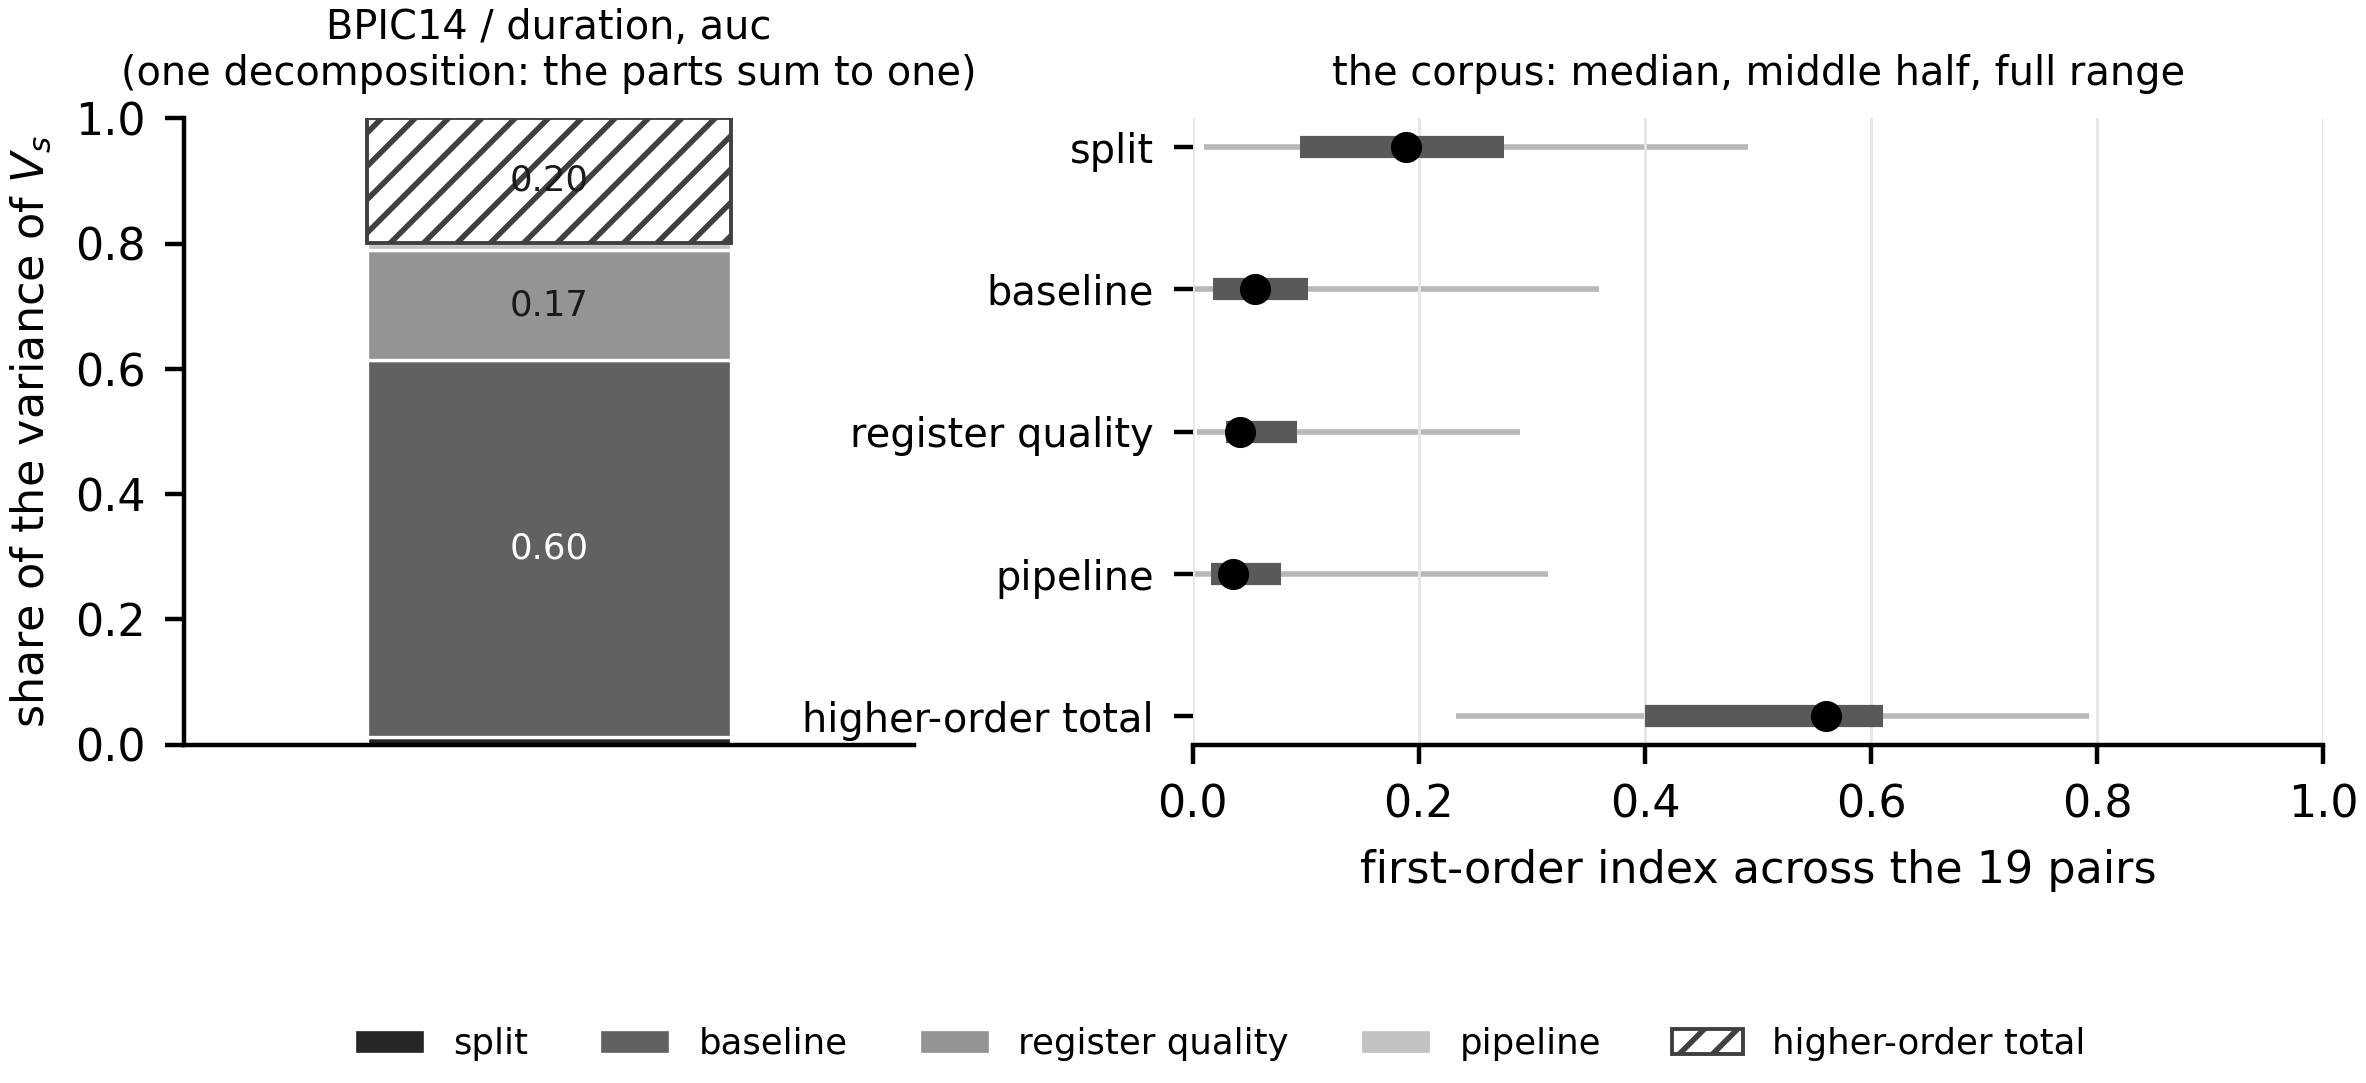
\includegraphics[width=\linewidth]{figS2_sobol.png}
\caption{The decomposition, within instrument, under the equal-level measure.
\emph{Left}: one pair at one instrument, so the components are a
decomposition and the parts sum to one exactly --- the largest pair in the
corpus, at the reference instrument, which is the cell every other table
reports at. The hatched segment is the total higher-order share
$1 - \sum_i S_i$ of~\eqref{eq:inttotal}. \emph{Right}: each axis's
first-order index across the corpus, as the median over pairs with the range
the middle half occupies and the full range. Nothing on the right is stacked,
because a median over pairs and a median over instruments do not add and a
stacked bar of them would invite the addition. The bootstrapped indices and
their intervals are in Table~\ref{tab:sobol}.}
\label{fig:sobol}
\end{figure}

Table~\ref{tab:sobol} and Figure~\ref{fig:sobol} give the decomposition,
computed within each instrument in that instrument's own units, under the
equal-level measure. The table's first four columns are, per pair, the median
over the five instruments of each axis's first-order index; its last column is
the largest per-axis interaction \emph{involvement}. Three aggregations of
this table are quoted below and they are not interchangeable, so each is named
where it appears: the median over pairs of a column of this table; the
\largestFirstOrderPct\ figure, which is the median over pairs of the median
over instruments of the \emph{per-instrument} largest first-order index, and
which is therefore not obtainable by taking a maximum across the four printed
columns; and the corpus medians of the higher-order share. The per-instrument
quantities the second is built from are in Table~\ref{tab:measures}.

\textbf{No single axis dominates, and the largest is the one an evaluation
paper is most likely to fix without comment.} Across the corpus the median
first-order index is \sSplitPct\ for the split, \sRungPct\ for the baseline
rung, \sQualityPct\ for the register-quality condition and \sLearnerPct\ for
the pipeline. The split leads the other three by a wide margin and still
explains well under a quarter of the variance. At the median pair the largest
of the four, whichever it is, is \largestFirstOrderPct.

\textbf{Most of the variance belongs to no single axis.} The total
higher-order share $1 - \sum_i S_i$ has median \interactionTotalPct\
(\interactionTotalCI\ over pairs), ranging from \interactionMinPct\ to
\interactionMaxPct; the largest per-axis \emph{involvement}
$\max_i (S_{T_i} - S_i)$ is a different quantity and is
\largestInvolvementPct\ at the median pair.

\textbf{The measure is not neutral, and one conclusion does not survive it.}
Across the three product measures the higher-order share moves by
\measureSpreadPct, and under the measure concentrated on the reference cell
it is \interactionTotalConcentratedPct\ --- smaller than the largest
first-order index under the same measure, \concentratedFirstOrderPct, on
\nConcentratedExceeds\ of \nPairs\ pairs. \emph{The interactions carry more
than any main effect} is therefore a claim about a measure and not only about
a surface. Supplement~\ref{app:measures} carries the target axis, which axis
leads on which pair, and both invariance tests.

\textbf{The baseline axis moves the answer by more than the answer.} Holding
the pipeline, the split, the register and the metric at the reference and
varying only the baseline rung, the increment moves by \spreadMedian\ AUC at
the median pair and \spreadMax\ at the widest --- larger than the increment
itself at the reference cell on \nSpreadExceedsIncrement\ of the \nPairs\
pairs. The index and the spread answer different questions, what share of the
\emph{variance} an axis explains while every other axis is also varying
against how far that one axis moves the answer on its own, and both are
reported because either alone misleads.

\paragraph{The pipeline axis is two axes} Its levels are a model family
together with an encoding and, in one case, a calibration, and on
\nPairsTwoLearners\ of the \nPairs\ pairs only two of them run. Crossed on the
case study's log --- both families against all three encodings on both
targets, \nPipelines\ complete factorial pipelines ---
\textbf{the encoding is the larger of the two}, \sEncodingPct\ of the variance
against the family's \sFamilyPct, with an interaction, \sFamilyEncodingPct,
as large as either main effect: the fused index is not the sum of two indices.
Supplement~\ref{app:secondary} carries the crossed decomposition. It has not
been re-run on the other \nPairsOther\ pairs, which Section~\ref{sec:lim}
records.

\subsection{Resolution regions, and the coverage they have}
\label{sec:regions}


\begin{figure}[t]
\centering
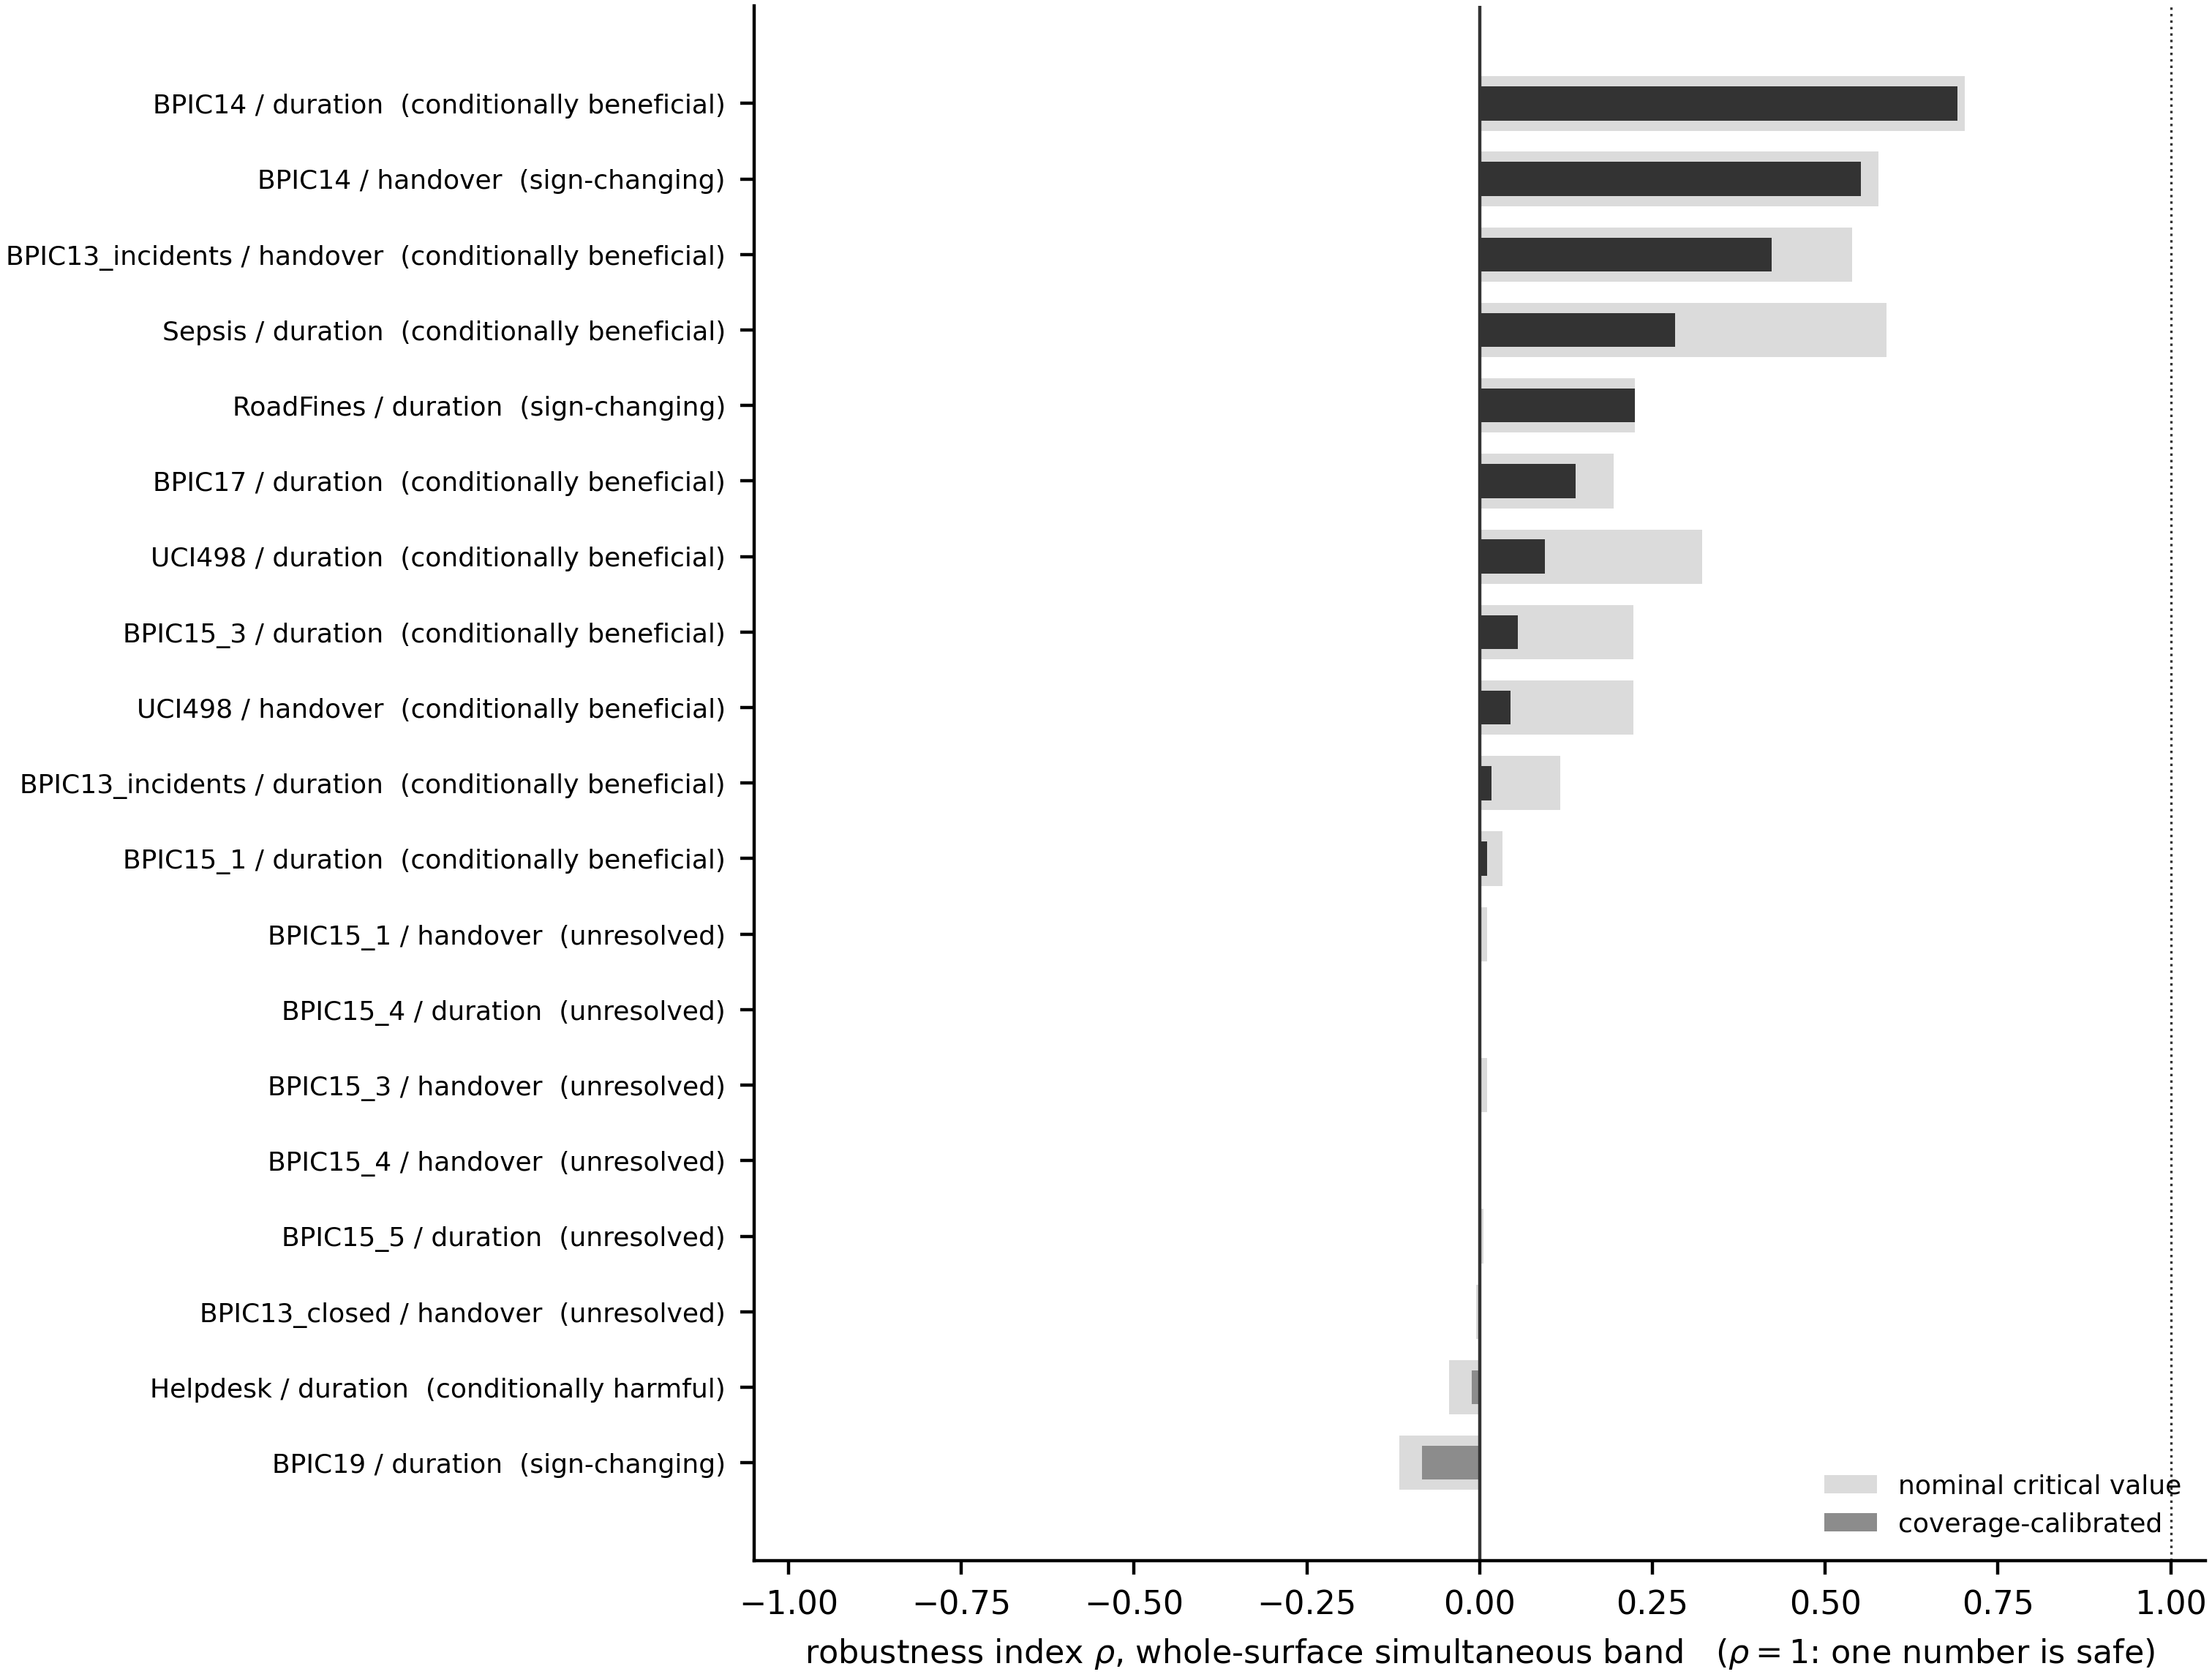
\includegraphics[width=0.92\linewidth]{figS3_regions.png}
\caption{The robustness index $\rho$ per log--target pair, with the region
label, under the coverage-calibrated critical value. $\rho = 1$, the dotted
line, is the only state in which a single positive number is a safe summary.}
\label{fig:regions}
\end{figure}

Table~\ref{tab:calbands} and Figure~\ref{fig:regions} carry the region labels
and the robustness index for every pair, computed on the inference surface
under the whole-surface simultaneous band at the conservative end of the
critical value's Monte Carlo interval. That family has a median
\familySizeMedian\ members per pair and a median critical value of
\maxTSurfaceMedian, against \maxTWithinMedian\ for a within-instrument family
and $1.96$ pointwise; under the narrower family the same draws give a
different region label on \nRegionChangedByFamily\ of the \nPairs\ pairs, and
the whole-surface family resolves \nResolvedWhole\ cells against the narrow
family's \nResolvedWithin.

\textbf{The nominal critical value is not enough, and the correction is
measured rather than assumed.} Section~\ref{sec:simsensitivity} shows that
coverage is governed by $K/n$ and that this corpus lives where coverage is
below nominal, the median pair sitting at \medianKoverN, so a region label
computed from a nominal band overstates how much of a surface is resolved.
The $(n, K)$ plane is dense enough to calibrate against, and
Supplement~\ref{app:calibration} derives the inflation factor $c(K/n)$ from it
--- a monotone regression through the measured factors, whose log-linear
summary has slope \calSlope\ (standard error \calSlopeSe). The factors the
corpus draws range from \calMin\ to \calMax; at the median pair the critical
value goes from \maxTSurfaceMedian\ to \qCalibratedMedian; the corpus resolves
\nResolvedCellsCalibrated\ cells against \nResolvedCellsNominal, a loss of
\resolutionLostToCalibrationPct, and \nRegionsChangedByCalibration\ of the
\nPairs\ region labels change. \textbf{Every region label and every $\rho$
quoted in this paper is the calibrated one}; Table~\ref{tab:calbands} prints
the nominal columns beside them.

\textbf{The factor's reach in $n$, and the two things widening the plane
found.} The plane is fitted at training sizes \planeNtrainLo\ to
\planeNtrainHi\ and this corpus runs \corpusNtrainLo\ to \corpusNtrainHi, so
all \nPairsInsidePlaneN\ of the \nPairs\ pairs lie inside the range the
factor is identified on. That is the arrangement a calibration needs, and it
is not the end of the matter.

\textbf{$K/n$ is not sufficient, and a plane wide enough in $n$ can now show
it.} Adding $\log n$ to the fit gives a coefficient of
\planeNdependenceBeta\ at $t = \planeNdependenceT$: at a fixed ratio the
widening a pair needs grows with its sample size. The design that isolates it
is the ladder, three ratios held fixed while $n$ moves over two orders of
magnitude, and along it the measured factor moves by \ladderSpreadMax\ ---
\ladderSpreadSE\ combined Monte Carlo standard errors --- while coverage
itself moves by \ladderCoverageSpreadPct. The applied curve is a function of
the ratio alone, so it carries that dependence as a residual: it sits below
the measured factor's own lower confidence limit on \nCellsUnderApplied\ of
the plane's cells, by at most \maxShortfallApplied, and both are large-$n$
cells. A two-covariate fit in $\log(K/n)$ and $\log n$ does not repair it
--- it is worse than the monotone curve on every cell-weighted criterion
(Supplement~\ref{app:calibration}) --- so the residual is reported rather
than fitted away.

\textbf{And on \nPlaneCellsUndefined\ of the \nPlaneCellsOffered\ cells the
factor does not exist at all.} The inflation factor is a widening \emph{about
the point estimate}, and Section~\ref{sec:boot} shows that past a crossing in
$n$ the basic interval stops containing the point estimate. Where it does,
there is no widening about $\hat{V}$ that attains nominal coverage and the
quantity this calibration estimates is undefined. All
\nPlaneCellsUndefined\ such cells are at \nStraddleHalfMin\ training rows or
more. The admission rule --- a cell enters the plane when the interval
straddles its estimate in at least \straddleMin\ of replicates --- decides
nothing: the rejected cells reach \straddleGapLo\ and the admitted ones start
at \straddleGapHi, so any threshold between those two gives this plane.
Section~\ref{sec:lim} carries what that leaves the corpus's largest pairs.

Under the calibrated band the region counts are: conditionally beneficial,
\nCondBeneficialCal; sign-changing, \nSignChangingCal; conditionally harmful,
\nCondHarmfulCal; unresolved, \nUnresolvedCalibrated; and the median
robustness index is \rhoMedianCalibrated.

\textbf{Of the \nPairsResolvingAny\ pairs that resolve anything,
\nCondBeneficialCal\ have no harmful cell and \nPairsResolveBothSigns\ resolve
cells of both signs.} That is the informative reading of the region column,
and it is the one to carry away: on two thirds of the pairs where the data
determine any sign at all, every sign they determine points the same way; on
the remaining third they do not.

\textbf{No surface in this corpus is uniformly beneficial, and that statement
is weaker than it looks.} It holds under the calibrated band, the nominal one
and the empirical one --- but \emph{uniformly beneficial} requires every
admissible cell's lower band to be above zero, and a cell whose point estimate
is negative can never qualify at any critical value. Every one of the \nPairs\
pairs contains at least one such cell, so the label is unreachable here before
any band, bootstrap or calibration is applied, and the count of zero is not an
inferential finding. The statement that carries content needs none of the
apparatus: on every pair at least one admissible specification has a negative
increment, which is visible from the all-cells column of
Table~\ref{tab:misreport}. What the apparatus earns is $\rho$ and the resolved
counts, not this. For the same reason $\rho = 1$ is not an attainable state
for any pair in this design, and Section~\ref{sec:regionsdef}'s remark that it
is the only safe state for a single number should be read as a definition
rather than as a hypothesis this corpus tests.

\textbf{The counts are reported at four settings, and the ordering is stable
across all of them.} At $c = 1$ --- the nominal band, no calibration at all
--- the corpus resolves \nResolvedSensNominal\ cells at a median $\rho$ of
\rhoSensNominal; under the calibrated factors, \nResolvedSensCalibrated\ cells
at \rhoSensCalibrated; pushing every factor to the upper end of its own Monte
Carlo interval, \nResolvedSensUpper\ at \rhoSensUpper; and under the
\emph{empirical} critical value of Section~\ref{sec:simbands} rather than the
multiplier one, \nResolvedWholeEmp\ against the multiplier's
\nResolvedWholeMult. That last comparison is not a calibration setting but a
different estimator of the same quantity, and it moves the resolution by more
than the calibration does. What moves across all four is how much resolution
the corpus has; what does not move is that no pair reaches $\rho = 1$. The
transfer from a pointwise interval in a simulation to a simultaneous band on
real logs, and the choice between the two critical-value estimators, are both
assumptions, and Section~\ref{sec:lim} carries them as limitations.

\subsection{What one number costs}
\label{sec:results-regret}


A conventional report --- one pipeline, the clean register, the single
holdout, ROC AUC --- disagrees in \emph{sign} with a median
\misreportEqualPct\ of the other admissible specifications under the
equal-level measure. Two things are wrong with reading that as \emph{what a
one-number report exposes a reader to}, and both are corrected before the
headline is stated.

\textbf{The axes are not all the same kind of thing.} The design space mixes
choices an analyst makes with things that are not choices at all, and
Table~\ref{tab:axiskind} partitions the decomposition accordingly:
\emph{analyst latitude} is the pipeline and the baseline rung;
\emph{resampling} is the split, five of whose six levels are expanding-origin
folds on the same data; \emph{counterfactual} is the register-quality
condition, a different state of the world rather than a different way of
analysing this one. On the primary scale, analyst latitude carries a median
\shareLatitudePct\ of the variance, resampling \shareResamplingPct\ and the
counterfactual \shareCounterfactualPct, and resampling is the larger of the
first two on \nPairsResamplingOverLatitude\ of the \nPairs\ pairs.

\textbf{Whether the split moves the increment more than the analytic axes
depends on which scale the partition is taken under, and we report both
rather than the one that reads better.} The primary scale decomposes
\emph{inside} each instrument and takes the median across the five, so the
instrument is a stratum and its own contribution is in none of the three
columns. Making it a sixth axis needs the headroom rescaling of
Section~\ref{sec:sobol}, because raw AUC and raw average precision do not
share units --- and on that scale the ordering reverses: analyst latitude
carries \shareLatitudeCrossPct, resampling \shareResamplingCrossPct\ and the
counterfactual \shareCounterfactualCrossPct, with resampling the larger on
\nPairsResamplingOverLatitudeCross\ pairs. The instrument is an analyst's
choice, so the second number is the one that answers the question as asked;
the first is the one taken on the units the rest of Section~\ref{sec:multilog}
uses. Neither is a corpus fact independent of the scale, which is the
paper's own thesis applied to the paper. Restricted
to the \nCellsLatitude\ analyst-latitude cells a pair carries, the
disagreement rate is \misreportLatitudePct\ against the pooled
\misreportEqualPct: the first is what a one-number report exposes a reader to,
the second what a claim ranging also over degraded registers and resampled
splits is exposed to.

\textbf{The reference specification is itself a choice, and moving it moves
the headline by less than the corrections above.} The rate counts cells whose
sign disagrees with the reference cell, so the reference supplies the sign
and nothing else. Varying it one axis at a time over every level that axis
carries --- \nRefSensVariants\ variants in all, Table~\ref{tab:refsens} ---
the corpus median runs \refSensMinPct\ to \refSensMaxPct\ against the
declared \refSensDeclaredPct: \refSensBoostingPct\ if the reference
pipeline becomes target-encoded boosting, and \refSensMetricMinPct\ to
\refSensMetricMaxPct\ across the five instruments. The headline is not an
artefact of which cell we called conventional.

\textbf{And most cells are not cells whose sign the data determine.} The
median pair resolves \nResolvedMedian\ cells of the \nCellsPerPairMedian\ it
carries, and sign agreement between two draws from a distribution centred near
zero is one half by construction, so a rate computed over unresolved cells is
partly measuring that.

\textbf{On the cells the corpus can resolve, the rate is
\misreportPooledResolvedPct.} Of the \nResolvedCorpus\ cells whose
coverage-calibrated whole-surface band excludes zero, \nDisagreeResolved\
disagree in sign with the reference cell. Every cell it counts is one where
the data do determine a sign, and that sign contradicts the number a
conventional paper would print.

\textbf{Applying both corrections at once gives
\misreportPooledResolvedLatitudePct, which is the number this section's own
argument asks for.} The two corrections above --- restrict to the axes an
analyst chooses, and restrict to the cells the band resolves --- were made
separately. Imposed together they leave \nResolvedLatitude\ cells, of which
\nDisagreeLatitude\ disagree. That is larger than the resolved-cell rate and
smaller than the analyst-latitude rate, and it is the rate that answers ``how
often would a one-number report be wrong about a sign that the data determine,
on a cell an analyst might actually have stood on''.

\textbf{Weighting by magnitude does not rescue the conventional report, and
the rate depends on the measure.} Weighting each cell by $|V|$ as well as by
the measure gives a median \misreportMagnitudePct, \emph{higher} than the
unweighted rate: the cells that disagree are not the negligible ones. The
median is \misreportEqualPct\ under the equal-level measure,
\misreportReferencePct\ under the reference-weighted and
\misreportConcentratedPct\ under the concentrated, falling as the measure
concentrates on the reference specification, which is what it should do. A
sign comparison is unit-free, which is why this one quantity may be pooled
across instruments where an expected loss may not.

Table~\ref{tab:regret} attributes the disagreement to axes. Holding everything
else fixed and changing one axis, the sign of the increment flips for a median
\flipSplitPct\ of same-everything-else pairs of cells under the split,
\flipLearnerPct\ under the pipeline, \flipRungPct\ under the baseline rung,
\flipQualityPct\ under the register-quality condition and \flipMetricPct\
under the metric. The two axes an evaluation paper is most likely to hold
fixed without comment --- which split, which pipeline --- are the two that
flip the sign most often.

\subsection{The eight pairs where the construct is what this paper is about}
\label{sec:family}

Every corpus statistic is reported on the \nItsmPairs\ ITSM-like pairs as
well as on all \nPairs\ (Table~\ref{tab:family}), because the register there
is a maintained one and the construct is what the paper is about.
\textbf{The headline is lower on the population this paper is about}: the
sign-disagreement rate is \misreportItsmPct\ against \misreportEqualPct\ over
the corpus, and on resolved cells \misreportPooledItsmPct\ against
\misreportPooledOtherPct\ on the rest. The decomposition barely moves ---
higher-order \itsmHigherOrderPct\ against \interactionTotalPct, largest
first-order \itsmLargestFirstOrderPct\ against \largestFirstOrderPct.
Supplement~\ref{app:itsmfamily} carries every statistic on both populations.

\subsection{Against specification-curve analysis as practised}
\label{sec:sca}

The closest existing practice is specification-curve analysis
\citep{simonsohn2020specification}: enumerate the reasonable specifications,
plot the curve, and test it against a sharp null by permutation.
Table~\ref{tab:sca} runs it unchanged on \emph{every} admitted pair ---
\nScaPairs\ of them, \nScaPerms\ permutations of a declared
\nScaCells-cell sub-surface --- beside the region label computed on the same
cells, which makes ``how often do the two verdicts part company'' a
measurement rather than an illustration. Two budgets are declared, the
sub-surface and a cap of \nScaMaxCases\ cases per pair that binds on
\nScaCapped\ of them; Supplement~\ref{app:secondary} gives both.

\textbf{They part company on \nScaDisagree\ of the \nScaPairs\ pairs}, close
to half. The permutation test rejects the sharp null --- the surface is
decisively unlike one with no signal --- and the same cells contain
increments of \emph{both} signs. A reader given only the test would conclude
that the register matters and have no way to learn that whether it helps or
hurts depends on choices nobody told them about. On \nScaAgreeNull\ pairs
neither resolves and the cheaper instrument suffices; the rest are mixed.

\textbf{And a specification curve is a statement about the cells it
enumerates.} On \nScaSubSurfaceDisagree\ pairs every cell of the sub-surface
has one sign while the \emph{full} surface is sign-changing or conditionally
harmful. Nothing is wrong with either --- they are claims about different
sets --- which is the point: without a declared denominator and a
simultaneous band, a curve cannot distinguish ``the sign holds'' from ``the
sign holds on the cells I drew''.

Neither subsumes the other. The permutation test answers \emph{is there
anything here}, costs one refit per permutation per cell and needs no band;
the region answers \emph{may I quote a sign}, costs a nested bootstrap, and is
what a reader deciding whether to act needs. This paper's contribution is the
second, and the first should be reported beside it.

\subsection{Decision rules, in sample and out}
\label{sec:rules}

The four rules of Section~\ref{sec:regretdef} are compared under the loss
defined there, inside one instrument at a time. Out of sample --- choosing on
a random half of the admissible cells and paying on the other half --- the
one-number rule costs \oosOneNumberAuc\ AUC of expected excess regret against
\oosMajorityAuc\ for the majority rule and \oosMeanAuc\ for the weighted
mean. \textbf{Three results run against the surface's advocate and we report
them}: the conservative rule is worst in \nInstrumentsUniformWorst\
instruments of \nInstruments, the one-number rule's median excess regret is
\emph{zero} in every instrument, and under rolling-origin folds the ordering
does not hold, at \oostOneNumber\ against \oostMajority. We therefore do not
conclude that a surface report is a better decision rule than a number; the
case rests on the decomposition and the sign disagreement, and this is a
check on those. Table~\ref{tab:rules} and Supplement~\ref{app:rulesdetail}
carry it.
% ---- paper/parts/50_cmdb.tex ----
\section{Case study: a configuration management database}
\label{sec:cmdb}

A configuration management database is the register an IT estate keeps of the
items it contains, and it is bought partly on the argument that operational
analytics need it. This section evaluates one against a named decision on a
public log: will this case be reassigned to another group before it is
resolved? The estate is a bank's and the log is BPI Challenge 2014
\citep{vandongen2014bpic}; the register field is the affected configuration
item, with \cardF\ distinct values. It is reported at greater length than the
other \nPairs\ pairs because it is the case that motivated the study and the
one on which the decision time --- when in the service-desk process the
prediction is made --- decides the answer.

\subsection{One log, two published answers, and what separates them}
\label{sec:cohort}


This log appears twice in this paper. Section~\ref{sec:multilog} applies the
registered generic rules of Section~\ref{sec:design}, which admit
\nRegisteredCohort\ cases and define the target by the registered handover
rule. This section uses the cohort and the reassignment target defined for the
estate: \nCohort\ cases at prevalence \casePrevalence\ (\casePrevalenceTest\
in the test half), \nCaseTrain\ in
training and \nCaseTest\ in test. The first set is a strict subset of the
second; the extra \nExtraCases\ cases are those the estate's own cutoff
excludes.

The two produce different answers about the register at the later decision
time, and the difference is large enough to change the sign. Against intake
plus group plus the knowledge reference, the estate's cohort and reassignment
target give \VTtwoKnow\ and the registered cohort and handover target give
\VregisteredTauTwo, on which the planned contrast \textsf{PC3}'s one-sided
$p$-value rejects at the Holm-adjusted level while its interval does not
exclude zero (Section~\ref{sec:planned}). Table~\ref{tab:cohort} takes the
manuscript from the first to the second one factor at a time.

\textbf{It is the target, not the cohort.} Over the cohort $\times$ target
design the target carries \shareTargetPct\ of the variance in the increment,
the cohort \shareCohortPct, and their interaction \shareCohortTargetPct.
Reassignment to another group before resolution has prevalence
\casePrevalence; handover between activity groups, under the registered rule,
has prevalence \prevRegisteredHandover. They are not the same question and the
register is not worth the same to them. Two further candidate explanations
were checked and are not explanations: the fields reached by the two analyses
agree on every row.

\textbf{An axis nobody declares, and this paper was standing on it.} Both
analyses sort the log in time and split at seventy per cent of the row order,
and \nTiedTimestamps\ incidents share their timestamp with another. How those
ties are broken decides which cases fall either side of the split, and the
sort the case study originally used was not stable, so its tie order was
neither declared nor reproducible: it printed \VpublishedTauTwo\ where the two
declared rules both give \VTtwoKnow. Over \nTiebreakDraws\ random tie-breaks
the increment at the knowledge rung ranges over \tiebreakRange\ AUC with a
standard deviation of \tiebreakSd, and it does not change sign
(\nTiebreakPositive\ of \nTiebreakDraws\ draws are positive), so no conclusion
here turns on it --- but it is a quarter of the point estimate's own
magnitude, produced by a choice no reporting standard asks anyone to state.
Every number in this section is computed under a declared tie-break, by
incident identifier, on the estate's cohort and reassignment target, and every
caption says so; the registered cohort's answers are in
Section~\ref{sec:multilog} with the other \nPairs\ pairs. The decision-time
result below is therefore a statement about a routing decision on this estate,
not about handover in general.

\subsection{Three decision times}
\label{sec:twodecision}


An incident in this estate does not begin as an incident. A caller reaches the
service desk, an \emph{interaction} is opened, the desk works it, and if it
cannot be closed there an incident is created and routed. Three moments at
which a prediction could be made are estimated, and what changes between them
is not only which fields are admissible (Table~\ref{tab:tau}).

\begin{description}
\item[$\tau_0$, first touch, every call.] The desk has just picked up the
call and does not yet know whether it will escalate. The population is every
interaction --- \nTauZero\ of them --- the register is the interaction's own
affected item, with \cardTauZero\ values, and the admissible baseline is the
interaction's intake block. Against it the register is worth \VtauZero\
[\VtauZeroLo, \VtauZeroHi].
\item[$\tau_1$, first touch, the calls that escalate.] The same moment and
the same fields, restricted to the \nTauOne\ calls that did become incidents.
The register is worth \VtauOne\ [\VtauOneLo, \VtauOneHi].
\item[$\tau_2$, incident creation.] The desk has worked the interaction and
escalated it. The population is the \nTauTwo\ incidents; the group that logged
the incident is known, and so --- probably --- is the knowledge-article
reference the desk consulted. Against the intake block the register is worth
\VtauTwo; against intake plus group, \VTtwoGroup\ [\VTtwoGroupLo,
\VTtwoGroupHi]; against intake plus group plus the knowledge reference,
\VTtwoKnow\ [\VTtwoKnowLo, \VTtwoKnowHi] --- the one rung of the five that
does not resolve.
\end{description}

The pairwise differences separate the mechanisms that a baseline ladder alone
conflates, and separating them properly requires one more row than the three
moments give. $\tau_1$ and $\tau_2$ are \emph{not} the same cases:
\nTauTwoUnmatched\ incidents have no interaction record, so $\tau_2$ carries
\nTauTwo\ cases against $\tau_1$'s \nTauOne. Table~\ref{tab:tau} therefore
also reports $\tau_2$ restricted to $\tau_1$'s own population --- the same
\nTauTwoMatched\ cases at the same prevalence \prevTauOne\ --- which is the
row that makes the information step an information step.

Restricting the population from every call to the calls that escalate, holding
the information fixed, moves the increment by \deltaCohortAtTau\ AUC. Moving
from first touch to incident creation \emph{on the matched cases}, changing
what is known and nothing else, moves it a further \deltaSnapshotAtTau. The
remaining \deltaPopulationResidual\ is what the \nTauTwoUnmatched\ incidents
with no interaction record are worth, and it is a population difference rather
than an information one: the unadjusted $\tau_1$-to-$\tau_2$ step,
\deltaSnapshotUnmatched, is the sum of the two and attributing all of it to
information would overstate the information channel by three quarters.
Admitting the group and then the knowledge reference takes the increment the
rest of the way to zero. A decision time is therefore an argument of the
estimand in its own right: it fixes the population, the feature snapshot and
the admissible set, and only the third of those is a baseline.

Neither $\tau_0$ nor $\tau_2$ is ``the'' answer: which one a reader wants
depends on where in their own process they intend to predict. A desk screening
at $\tau_0$ looks at \nTauZero\ calls a year at a prevalence of \prevTauZero;
a desk screening at $\tau_2$ looks at \nTauTwo\ incidents at \prevTauTwo, and
Section~\ref{sec:nbregret} prices the difference.

\subsection{The leakage tipping point, and register quality}
\label{sec:quality}

Two further experiments on this estate are in Supplement~\ref{app:casedetail}
and summarised here.

\textbf{A field that looks like leakage has a tipping point, and where it
sits is what a reader has to judge.} The knowledge reference is the field
that takes the register's increment to indistinguishable from zero, and
whether it was available at $\tau_2$ is probable but unproven. Writing
$\lambda$ for the share of its values assumed written \emph{after} the
incident --- so that a larger $\lambda$ makes more of the field inadmissible
--- the register is worth \VTtwoKnow\ [\VTtwoKnowLo, \VTtwoKnowHi] at
$\lambda = 0$, not resolvably different from zero, and reaches half of its
knowledge-free value at $\lambda = \lambdaHalf$. A reader who believes more
than \lambdaHalfPct\ of references are written after the incident should read
this estate's register as worth at least half of \VTtwoGroup\ AUC, and one
who believes almost none are should read it as worth almost nothing. We
cannot measure $\lambda$, so the disposition of an unprovable admissibility
assumption is reported as a sensitivity analysis and not as a headline
(Figure~\ref{fig:tipping}, Table~\ref{tab:tipping}).

\textbf{Register quality is an axis, not a caveat, and which rows go missing
matters as much as how many.} Under \nQualityKinds\ declared degradation
mechanisms the increment at the reference cell moves from \qClean\ on a clean
register to \qRareHalf\ when half the population is lost from its long tail
and \qCommonHalf\ when half is lost from its core. Three of the mechanisms
are \emph{dependent} --- on time, on content, and on a training-estimated
propensity that correlates missingness with the outcome --- and they carry
severity integrals \integralTime, \integralContent\ and
\integralPropensity\ against \integralMaskRare\ for the independent long-tail
mechanism, which they bracket rather than track. A quality axis built only
from independent coin flips measures one corner of the question.
Tables~\ref{tab:quality2} and~\ref{tab:quality3} carry every mechanism and
level.

\subsection{What this says to a configuration management programme}
\label{sec:csdm}

The register in this log is layered, and the layers are the ones a common
service data model uses: an item belongs to a class, a class to a subtype, and
a subtype rolls up to a service component. Supplement~\ref{app:layers}
estimates the increment at each layer against the intake block, on the
registered targets. The coarse layers are \emph{not} free --- on the handover
target the item's type alone is worth \layerTypeHandover\ and its subtype
\layerSubtypeHandover, against \layerItemHandover\ for the item itself, and on
duration \layerTypeDuration\ against \layerItemDuration\ --- so knowing that a
case concerns \emph{a laptop} is worth between a third and two thirds of
knowing which one. What the item adds \emph{on top of} the subtype is the
quantity a populated hierarchy does not buy, and it is
\layerItemMarginalHandover\ on handover and \layerItemMarginalDuration\ on
duration. A programme that populates the class hierarchy and stops has bought
a real part of the value and left the larger marginal part on the table; it
has not bought nothing. These figures are on the registered targets rather
than this section's reassignment target, and Supplement~\ref{app:layers} says
so.

The three dependent quality mechanisms map onto how a configuration management
database actually decays, which is why they are in the design space rather
than independent coin flips. \emph{Discovery lag} is the interval between a
service going live and the discovery tooling finding its items, which is why a
new service's cases carry an empty affected item for weeks. \emph{Unreconciled
duplicates} arise when two discovery sources write the same physical item
under two identifiers. \emph{Propensity-dependent missingness} arises when the
affected item is populated by the desk rather than by discovery: the unusual
case, which is the one worth predicting, is the one the desk is least likely
to classify correctly under time pressure. The measured costs above say which
of the three is worth spending on: on this estate, coverage and accuracy at
the item level, and not reconciliation.

Two disclaimers. This is predictive performance on one estate for one
decision, not procurement advice, and a register that pays nothing here may be
bought for change control, audit or impact analysis, none of which this
measures; and the ranking of the mechanisms is a property of this cohort's
cardinality and volume.

\subsection{The absorption, and why the ratio is secondary}

The quantity a report of this kind usually leads with is the \emph{relative}
reduction $R$: the share of the register's apparent value that a single free
field absorbs. The absolute absorption $D = V(f \mid B_0) - V(f \mid B_1)$ is
reported first, with its own interval, and $R$ second with a Fieller set and
the set's kind. On this estate at the reference cell $D$ is \Dabs\ [\DabsLo,
\DabsHi] and $R$ is \Rref\ with a \RrefKind\ Fieller set;
\nFiellerUnboundedCase\ of the \nFiellerCase\ reductions this ladder produces
have a Fieller set that is not a bounded interval, and for those a percentile
interval is not a summary of anything. Across the corpus the figure is
\nFiellerUnbounded\ of \nFieller, and the full ladder is
Table~\ref{tab:absorption}.
% ---- paper/parts/60_dca.tex ----

\section{Decision-analytic evaluation}
\label{sec:dca}

An increment in AUC is not a quantity a service desk can act on. This section
reads the same surface in net benefit, which is: the number of correctly
nominated cases per thousand arrivals, net of the false nominations, at a
declared exchange rate between the two.

\subsection{The operating point is a cost ratio, not a knob}

At threshold $\theta$ the net benefit of a rule that nominates when
$\hat p \geq \theta$ is
\[
\mathrm{NB}(\theta) \;=\; \frac{\mathrm{TP}(\theta)}{n}
\;-\; \frac{\mathrm{FP}(\theta)}{n}\cdot\frac{\theta}{1-\theta},
\]
so $(1-\theta)/\theta$ is the number of false nominations the desk is willing
to accept for one true one. Choosing $\theta$ is choosing an operational cost
ratio, and it belongs to the analyst's declaration rather than to a grid
search. We report the whole grid --- \nGrid\ points from \gridLo\ to
\gridHi\ --- and name three points a desk might occupy: $\theta =
\thetaCheap$, or \ratioCheap\ false nominations accepted per true one, where a
review is cheap and the desk nominates liberally; $\thetaBase$, or
\ratioBase, where a review and a miss cost about the same; and $\thetaDear$,
or \ratioDear, where review capacity is scarce. A reader whose desk sits at a
ratio not in that list reads their own point off Figure~\ref{fig:dca}: the
operating point is the reader's to choose, so the analyst reports the curve
rather than a point on it.

\subsection{Calibration comes first, or the threshold means nothing}
\label{sec:calibfirst}

A threshold is a statement about probability, so a model whose probabilities
are wrong is being read at a threshold it does not have. Every decision curve
here is therefore computed on \emph{calibrated} scores, with the calibrator
fitted inside the training half and rebuilt inside every bootstrap refit, and
a registered rule excludes an arm whose calibration slope leaves
$[0.5, 2]$. Supplement~\ref{app:dcadetail} gives the rule, what it removes and
what the curves look like without it.

\subsection{Simultaneous bands change what can be said}
\label{sec:dcabands}

The decision-curve family is declared separately from the scalar surface and
carries its own max-$t$ critical value, because net benefit and a scalar
instrument are not the same scale. Across the \nDcGrid\ operating points of
this estate's curve \textbf{the pointwise interval declares the increment
resolvably positive at \nBeneficialPointwise\ of them and the simultaneous
band at \nBeneficialSimultaneous}, and the harmful counts are
\nHarmfulPointwise\ against \nHarmfulSimultaneous. Both are built from the
same draws, so the only thing that differs is the family: those points are
the price of a statement about a \emph{range} of thresholds rather than about
each one separately, and a paper that reads a decision curve across its range
while pricing it pointwise has claimed the first and paid for the second.

\textbf{This family is also the one most exposed to how the critical value
was estimated.} It is \emph{not} coverage-calibrated --- the $(n,K)$
calibration of Section~\ref{sec:regions} is estimated for the scalar family
--- and Section~\ref{sec:simband} finds that the widening it would need is
about twice what the surface families need.
Supplement~\ref{app:dcabandsfull} carries the comparison, the dip near
$\theta = \dcaDipTheta$ and Figure~\ref{fig:dca}; Table~\ref{tab:dca} prints
the curve.

\subsection{The decision, in units a service desk uses}
\label{sec:nbregret}

The comparison is run in net benefit per thousand cases, over a declared
distribution of exchange rates a desk plausibly holds
(\deskQlo\ to \deskQhi, centred \deskQmid), and only on models that pass the
registered calibration rule --- which excludes \nModelsDcaExcluded\ of
\nModelsDca\ arms and \nPairsDcaExcluded\ of \nPairs\ pairs.
\textbf{That count is itself the strongest operational finding here}: a
decision curve read off a model whose probabilities are wrong is read at a
threshold the model does not have.

\textbf{And the rules mostly tie.} The one-number rule's expected excess is
\excessOneNumberDesk\ per thousand against the conservative rule's
\excessUniformDesk, the four rules separate on only \nSeparatingDesk\ of
\nPairs\ pairs, and the one-number rule is worst on \nOneNumberWorstDesk.
\textbf{The case against one-number reporting does not rest on this design.}
What does separate in this unit is the decision time: the register promises
\promisedPerThousand\ per thousand at the earlier moment and delivers
\deliveredPerThousand\ at the later one, a shortfall of
\shortfallPerThousand. Supplement~\ref{app:deskfull} carries the rules, the
exchange-rate distribution and the exclusions; Tables~\ref{tab:desk}
and~\ref{tab:rules} the numbers.
% ---- paper/parts/70_standard.tex ----

\section{A reporting standard, and software}
\label{sec:standard}

\subsection{The minimum reportable form}

The apparatus of Sections~\ref{sec:surface} and~\ref{sec:inference} implies a
reporting standard short enough to state in full. A feature-value claim is
reportable when it carries: \textbf{the design space}, as an enumerable
declaration of which learners, encodings, targets, splits, decision times,
quality mechanisms, baselines, metrics and operating points are admissible,
why anything defensible was left out, and \emph{the measure placed on those
levels}; \textbf{the denominator}, as a count a reader can reproduce from the
axis levels --- declared cells, computed cells, and the cells any inference
actually rests on, which need not be the same set; \textbf{the absolute
increments} at every rung of the baseline ladder, in the metric's own units,
with intervals from a resampling scheme that refits the model; \textbf{the
sensitivity decomposition}, with the total higher-order share reported as
$1 - \sum_i S_i$ and not as any per-axis difference; \textbf{the resolution
region and $\rho$}, under a band whose family is the set the label ranges
over; and \textbf{the ratio $R$ last if at all}, with a Fieller set and the
set's kind, never where the denominator is not resolvably positive. Nothing
in that list is expensive once the surface exists, and the surface is a
factorial over declarations the analyst has already made implicitly.

\subsection{\texttt{fieldvalue}}
\label{sec:tool}

The standard ships as \texttt{fieldvalue}, which computes the surface from a
data frame, a feature name and a dictionary of baselines. Its notable
property is a refusal: \texttt{Surface} raises rather than returning a
scalar, \texttt{Surface.report()} emits the form above, and
\texttt{Surface.at(...)} returns one cell only if the caller names every
axis. Version \fvVersion\ adds the four objects of
Sections~\ref{sec:sobol}--\ref{sec:regretdef} as functions of a surface ---
\texttt{decompose}, \texttt{regions}, \texttt{robustness}, \texttt{regret}
--- each taking a tidy frame rather than this package's own object, so they
apply to a surface computed by some other pipeline. It carries \nTests\ tests
and is an \emph{independent implementation}: the analysis scripts and the
package compute the same four objects from the same definitions in different
code, neither written against the other, and on this corpus they agree on
\nAgreeQuantities\ of \nAgreeQuantities\ quantities to \agreeTolerance.

\subsection{Beyond process logs, and beyond this paper's claims}
\label{sec:worked}

The standard is not about event logs and not about configuration databases.
Supplement~\ref{app:worked} runs it on UCI Adult, where the expensive field is
\texttt{occupation} and the cheap ones come with the sampling frame: over
\exCells\ cells the reduction runs \exRmin\ to \exRmax; the baseline and the
metric carry the same share of the variance to three figures,
\exSbaselinePct\ and \exSmetricPct, against \exSpopulationPct\ for the
register population; and a one-number report misstates the sign for a mean
\exMisreportPct\ of the other cells. \texttt{examples/worked\_example.py}
produces all of it in \exampleLines\ statements against the package's public
interface.

\paragraph{How the surface is reported today}
\label{sec:practice}
Whether the axes this paper varies are varied in published work deserves a
systematic review, and we did not conduct one. A machine-assisted prevalence
pilot was run on a convenience frame and is \emph{not} reported here: with one
adjudicator, no independent human reliability study and a mechanical screen
whose measured sensitivity is \auditSens, it can generate a hypothesis about
practice and cannot test one. Its frame, sample, codes, adjudications and
evidence dossiers are in the archive. The paper's argument does not need it:
the case against one-number reporting is made by the decomposition and the
sign disagreement, on data, and not by a count of how often other authors
report one number.
% ---- paper/parts/75_simulation.tex ----
\section{Simulation against a known answer}
\label{sec:sim}

Everything so far has been measured on real logs, where the answer is not
known. This section measures the estimator where it is. The full tables are in
Supplement~\ref{app:tables} and the diagnosis of the one world that failed is
in Supplement~\ref{app:noisy}.

\subsection{Six worlds, two estimands}
\label{sec:simworlds}

The simulation uses \nWorlds\ worlds --- four of them misspecified for the
estimator --- at \nSimReps\ replicates each, with the covariate space finite
so that the population AUC of any scoring rule is computed in closed form
rather than simulated. Two estimands are separated because under
misspecification they differ: $V_{\mathrm{oracle}}$, the increment between
the two Bayes-optimal rules, and $V_{\mathrm{limit}}$, the increment between
the two fitted pipelines' limits. A resampling interval can only cover the
second, and reporting its coverage of the first as the estimator's coverage
is a category error. Supplement~\ref{app:worlds} describes the worlds and the
marginalisation a corrupted register forces; Table~\ref{tab:sim31} reports
both estimands.

\subsection{Coverage, bias and width}
\label{sec:simcoverage}

Coverage estimates carry a Monte Carlo standard error of about
$\simCoverageSE$ percentage points at \nSimReps\ replicates, which is the
resolution every comparison here should be read at;
Figure~\ref{fig:coverage} draws them by construction and world.

\textbf{Where the refit helps.} The nested basic interval covers at least as
well as the fixed-model percentile interval on \nWorldsNestedAtLeastNaive\ of
the \nWorldsSim\ worlds, and its median across them is
\coverageNestedBasicMedian\ against the fixed-model interval's
\coverageNaiveMedian. Both fall a little short of nominal on most worlds, by
more than the Monte Carlo resolution.

\textbf{Where the percentile interval fails, and why.} On the sparse world it
collapses to \coverageSparsePct, and the \emph{nested} percentile interval is
worse there than the fixed-model one. The cause is Section~\ref{sec:boot}: a
bootstrap training resample holds about $63\%$ of the distinct register
levels, so every refit sees a sparser register and the bootstrap distribution
shifts below the estimate. The basic interval pivots that shift out and
restores coverage --- \coverageSparseBasic\ --- and costs nothing where there
was nothing to repair, at a median \coverageNestedBasicMedian\ and a minimum
\coverageNestedBasicMin\ across all \nWorlds\ worlds. The bias-corrected
percentile does \emph{not} repair the sparse world (\coverageSparseBc), which
is why every interval and band in this paper uses the basic construction. The
$m$-out-of-$n$ subsampling interval, the standard alternative in exactly this
regime, does not win either: \coverageSparseMofn\ on the sparse world and a
median \coverageMofnMedian\ across the \nWorldsMofnPriced\ worlds it was
priced on.

\textbf{What no interval repairs.} Against $V_{\mathrm{oracle}}$ rather than
$V_{\mathrm{limit}}$, every construction undercovers on the drifting world ---
\coverageDriftOracle\ at best --- and it should: when the coefficients move
between eras the estimator is not consistent for the oracle quantity, and the
largest gap is \biasOracleMax\ in AUC units. Under misspecification an
interval around the estimator's own limit is not an interval around the
quantity a reader cares about, and no resampling scheme repairs that.

\subsection{Sample size, register cardinality and block length}
\label{sec:simsensitivity}

A construction that works at one sample size, one register cardinality and one
block length has been validated at a point, not in a regime. Sample size and
register cardinality are therefore varied \emph{jointly}, up to $K = \simKMax$
levels --- the cardinality of the case study's own register --- and the block
length is varied around its rule of thumb.

\textbf{The ratio $K/n$ captures most of the dependence, and not all of it.}
Across the plane the basic interval covers a median \coverageGridMedian\ and a
minimum \coverageGridMin, the last at a ratio of \simGridWorstRatio. Below
$K/n = \simGridRatioSafe$ its coverage lies between \coverageGridSafeMin\ and
\coverageGridSafeMax\ --- short of nominal everywhere, by about one Monte
Carlo standard error at \nPlaneGridReps\ replicates --- and it has fallen
below three quarters by \simGridRatioBad. The ratio is the right first-order
summary --- the mechanism of Section~\ref{sec:boot} is why, and
varying $n$ alone would not have exposed the regime the corpus occupies ---
but it is not sufficient, and the plane says so in two places. The two cells
closest to each other in ratio --- a register of \simGridSameRatioKa\ levels
at \simGridSameRatioNa\ training rows, and one of \simGridSameRatioKb\ at
\simGridSameRatioNb\ --- cover \simGridSameRatioCovA\ and
\simGridSameRatioCovB, a gap of \simGridSameRatioGapSE\ combined Monte Carlo
standard errors; and holding the register at \simGridFixedK\ levels while
moving the training half from \simGridFixedNa\ rows to \simGridFixedNb\ moves
coverage from \simGridFixedCovA\ to \simGridFixedCovB, so $n$ carries signal
of its own. The calibration of Section~\ref{sec:regions} is a function of the ratio
alone and therefore inherits this residual, which
Section~\ref{sec:lim} states.

\textbf{Where this corpus sits, and what is done about it.} The median
log--target pair here has $K/n = \corpusRatioMedian$, the range runs
\corpusRatioMin\ to \corpusRatioMax, and \nPairsRatioAboveTenth\ of \nPairs\
pairs are above a tenth. Most of this corpus therefore sits at or beyond the
ratio at which coverage starts to fall, and a nominal band on those pairs is
\emph{narrower} than a $95\%$ interval should be --- the anti-conservative
direction, which inflates the count of resolved cells. The plane is dense
enough to calibrate against, and Section~\ref{sec:regions} does.

\textbf{Where the interval stops containing its own estimate.} The denser
plane the coverage calibration of Section~\ref{sec:regions} is fitted on ---
a different and larger object from the \nSimGridCells-cell grid above, at
\planeNtrainLo\ to \planeNtrainHi\ training rows --- locates the crossing
Section~\ref{sec:boot} describes. At a fixed ratio
of \straddleRatio\ the basic interval straddles its own point estimate in
every replicate up to \nStraddleAllMax\ training rows and in only
\shareStraddleAtHalfPct\ of them by \nStraddleHalfMin, because the bootstrap
displacement is a bias that does not shrink with $n$ while the half-width
does. Past that crossing the inflation factor is not defined --- it is a
widening about the estimate, and there is nothing to widen about --- and
\nPlaneCellsUndefined\ of the plane's \nPlaneCellsOffered\ cells have none
for that reason, every one of them at \nStraddleHalfMin\ rows or more.
Section~\ref{sec:regions} reports what that leaves the corpus, and
Supplement~\ref{app:calibration} describes that plane's design.

\textbf{Block length.} \nSimBlockLengths\ lengths are examined --- half the
rule $\lceil n^{1/3} \rceil$, the rule, and twice it. Coverage moves with the
length, spanning \coverageBlockSpreadMax\ within a world, of the order of two
standard errors; but the comparison the paper rests on is unchanged at every
length, the basic interval beating the percentile interval on the sparse
register by at least \blockSparseGapMin\ at all \nSimBlockLengths.

\subsection{The band's family-wise coverage}
\label{sec:simband}

Everything above validates a \emph{pointwise} interval. Two of this paper's
four reporting objects are functions of a \emph{simultaneous} band, and until
this section nothing measured what that band covers.

\textbf{The design, and why its answer is an upper bound.} The truth is zero
at every cell of a synthetic family. One draw from the sampling distribution
gives the point estimate, and as many further draws \emph{from that same
distribution} as the corpus family it is matched to carries give the
bootstrap --- so the bootstrap is not an approximation of the sampling
distribution but is it. Every way a
resampling scheme can be wrong --- dependence it fails to reproduce, a refit
that comes apart, a block length misjudged --- is switched off, and what is
left is the object under test: a standard error and a critical value both
estimated from the same handful of draws. A coverage measured here is
therefore the most the real procedure can attain, and a shortfall here is one
that no improvement to the resampling repairs. The families are matched to
this corpus in size, draw count, cross-cell correlation, effective rank and
per-cell excess kurtosis; the matching is fitted by grid search against the
corpus's own draw files and reported beside its target rather than asserted.
Coverage is over \nBandCoverageReps\ replicates in each of
\nBandCoverageCells\ cells, so no coverage here is determined worse than
\bandCoverageSEMax.

\textbf{Three regimes, because ``the draws are heavy-tailed'' turned out to
name two different things.} Under \emph{Gaussian} draws the multiplier's
family-wise coverage is a median \covMultGaussMedian\ and a minimum
\covMultGaussMin. Under draws carrying this corpus's tails, whose median
cell has an excess kurtosis of \corpusKurtMedWhole\ on the surface families
and whose ninetieth percentile is \corpusKurtNinetyWhole, the median is
\covMultHeavyMedian\ and the minimum \covMultHeavyMin. Under the third
regime, which adds the degenerate cells described below, they are
\covMultDegenMedian\ and \covMultDegenMin.

\textbf{What is wrong with the decision-curve families is not a tail.} At a
threshold where both arms treat every case alike the net-benefit difference
is zero by arithmetic rather than by estimation, and \nDegenerateCellsDca\
cells of the corpus's curve families are exactly zero in at least nine draws
of ten --- up to \shareDegenerateDcaMaxPct\ of a single family, against
\nDegenerateCellsWhole\ such cells anywhere in the surface families. The
admission rule keeps any cell whose spread exceeds a floor in absolute units,
so such a cell survives and standardising it by that spread sends its
studentised value to the largest value a deviate standardised over $B$ points
can take. They are what makes $q_{\mathrm{emp}}$ large on those families:
excluding them moves the median ratio $q_{\mathrm{emp}}/q$ from
\ratioDcaAll\ to \ratioDcaAdmissible. It does \emph{not} dissolve the
disagreement --- $q$ still lies below the empirical interval on
\nQbelowEmpDcaAdmissible\ of the \nFamiliesDca\ curve families and
\nQbelowEmpWholeAdmissible\ of the \nFamiliesWhole\ surface ones once they
are gone --- and Table~\ref{tab:bandcov} reports the regime with and without
them because Section~\ref{sec:simbands}'s count of what
$q_{\mathrm{emp}}$ resolves is, on those families, partly a count of
arithmetic.

\textbf{How far short, in the units the calibration works in.} A critical
value is widened multiplicatively, so the useful summary of the shortfall is
the factor that would have closed it. On the surface families that factor is
\shortfallWholeMin\ to \shortfallWholeMax; on the decision-curve families,
\shortfallDcaMin\ to \shortfallDcaMax. The coverage calibration of
Section~\ref{sec:regions} applies \calFactorMin\ to \calFactorMax, is
fitted to restore \emph{pointwise} coverage rather than this one, and is
applied to the surface families only --- so it is of the right order where it
acts and absent where the shortfall is largest. Section~\ref{sec:lim} says
what follows.

\textbf{The draw count is the binding constraint.} At the modal surface
family the multiplier band covers \covMultBootThirtyThree\ at
\nBootThirtyThree\ draws and \covMultBootOneThousand\ at
\nBootOneThousand, and the per-cell interval underneath it moves
\covPercellBootThirtyThree\ to \covPercellBootOneThousand\ over the same
range: part of what the band loses it loses before any critical value is
chosen, and Section~\ref{sec:simcoverage} validated that construction at a
refit count this corpus does not reach on most pairs. No estimator recovers
the difference. The best of the five, the empirical quantile at the upper end
of its own order-statistic interval, reaches \covEmpHiHeavyMedian\ at
\widthEmpHiOverMult\ times the width and still falls to
\covEmpHiHeavyMin\ at the smallest family; a Rademacher wild multiplier,
which preserves the observed draws' magnitudes instead of replacing them by
Gaussians and is the natural repair for a tail problem, is worse than the
Gaussian multiplier at \covRadHeavyMedian.

\paragraph{What the simulation does not establish}
It certifies the pointwise constructions on \nWorlds\ worlds, a plane of
\nSimGridCells\ $(n, K)$ cells and \nSimBlockLengths\ block lengths, and
the band on the \nBandCoverageCells\ matched families of
Section~\ref{sec:simband} --- on nothing else. The stationarity and mixing the moving-block bootstrap needs are
assumed and not tested; the split point is fixed within a draw, so
split-position uncertainty is outside every interval reported here; and the
drifting world shows what happens when the estimator is not consistent for the
quantity a reader cares about.
% ---- paper/parts/80_limits.tex ----
\section{Limitations}
\label{sec:lim}

\paragraph{This is predictive performance, not value}
Nothing here measures what a register costs to acquire or maintain, whether
acting on a prediction changes an outcome, or what a data programme is worth.
The quantity is an increment in predictive performance, read at a declared
exchange rate in Section~\ref{sec:dca}. A reader who converts
Table~\ref{tab:master} into a procurement decision is doing something this
evidence does not support.

\paragraph{The design space is declared, not complete, and one omission is
structural}
$\mathcal{S}$ has \nAxes\ axes here. It could have more --- hyperparameter
tuning protocol, missing-data treatment for the baseline fields, the horizon
of the target, the label-noise model --- and the cohort rule is varied only on
the case study's log, so the honest form of the claim is ``the increment moves
this much over \emph{this} space''. The structural omission is that
\textbf{prefix length, prefix bucketing and sequence encoding are not axes
here and cannot be}, because this study predicts at one prediction point from
creation-time attributes. Those are the axes predictive process monitoring
varies most, so the corpus result measures sensitivity in a simpler adjacent
setting on the same data rather than in that literature's own benchmark, and
adding a prefix axis on at least one log is the clearest next study this paper
implies.

\paragraph{The axes are not all the same kind of thing}
Three of the nine are choices an analyst makes, one is a resampling scheme and
one is a counterfactual state of the register, and a variance decomposition
that pools them answers a question nobody asked.
Section~\ref{sec:results-regret} partitions them and reports the
sign-disagreement rate on the analyst-latitude sub-space
(\misreportLatitudePct) beside the pooled one (\misreportEqualPct). The region
labels and $\rho$ are \emph{not} partitioned, and are therefore conditional on
the quality axis being averaged over: a surface is asked to be resolvably
beneficial in cells where three quarters of the register has been deleted,
which is part of why no surface here is uniformly beneficial.

\paragraph{The inference surface is smaller than the declared surface, and the
grid is not uniform across the corpus}
Every point estimate comes from the full declared space; every \emph{band}
comes from the inference surface, a median \inferenceShareMedianPct\ of each
pair's computational surface. It is a subset of the declared surface cell for
cell and the share of positive cells differs between them by a median
\repGapMedian, but a study with compute to spare should equate the two. The
same budget shows in two further places. The draw counts run
\nDrawsSurfaceMin\ to \nDrawsSurfaceMax\ as declared and
\nDrawsEffectiveMin\ to \nDrawsSurfaceMax\ effectively, because a replicate
that leaves any cell of a family without outcome variation is dropped from
that family; the two families that lose the most sit on logs that also supply
much of the sign disagreement of Section~\ref{sec:results-regret}, so the
headline's largest contributors are also its noisiest. And the pipeline axis
carries four levels on the case study's log and two or three elsewhere, by a
rule declared on row count before the runs, so a sensitivity index computed on
one pair is not strictly comparable with one computed on another.

\paragraph{Every weighted quantity depends on a measure that is a modelling
choice}
A decomposition, a robustness index and a regret are all taken with respect to
a distribution over specifications, and there is no neutral one. Three product
measures and an envelope over a fourth are reported
(Table~\ref{tab:measures}); across the three the total higher-order share
moves by \measureSpreadPct. \textbf{One qualitative conclusion does not
survive all four}: under a measure concentrated on the reference
specification, a single axis carries more variance than everything
higher-order combined on \nConcentratedExceeds\ of \nPairs\ pairs, so ``the
interactions dominate'' is a claim about a measure and not only about a
surface. Two structural invariances, to duplicating a level and to refining a
grid, are enforced and tested, so no number here can be moved by re-describing
the same design space. Separately, the decomposition inherits the metric's
scale (Proposition~\ref{prop:scale}), which is why the within-instrument
decomposition is primary and the cross-instrument one is a sensitivity
analysis.

\paragraph{One estate for the case study, and a heterogeneous corpus}
The configuration management database analysis is one bank's estate, on one
public log, and the availability question at its centre is settled by
probability rather than by a timestamped field-value history; the strongest
version of this study would have an organisational partner supplying
timestamped field histories, a known prediction time, historical register
population and accuracy, and operational review costs. The \nPairs\ pairs are
also not replications of one another: across the \nLogs\ logs the two
registered targets label the same case identically on a median
\targetAgreement\ of cases. Every corpus-level statistic is therefore about
\emph{sensitivity}, and every one is reported on the ITSM family as well as on
the whole corpus (Table~\ref{tab:family}).

\paragraph{The quality mechanisms are synthetic}
Population loss, identity error, reconciliation failure and staleness are
constructed from the training half, not observed. Three of them are
\emph{dependent} --- on time, on the item's recorded type, and on a
training-estimated propensity that correlates missingness with the outcome ---
which is closer to how a register degrades than an independent coin flip, and
every one is verified by execution to read no test outcome. But a constructed
mechanism is not an observed one, and validating them against a genuinely
incomplete register is the obvious next study.

\paragraph{The coverage calibration is no longer an extrapolation in $n$, and
what replaced that problem is worse}
The plane that identifies the inflation factor is estimated at training sizes
\planeNtrainLo\ to \planeNtrainHi\ against a corpus running \corpusNtrainLo\
to \corpusNtrainHi, so every one of the \nPairs\ pairs now lies inside the
range the factor is identified on. Two things took the place of the
extrapolation.

\textbf{The applied curve is misspecified, measurably.} $\log n$ enters the
fit at $t = \planeNdependenceT$ (Section~\ref{sec:regions}): at a fixed ratio
the widening a pair needs grows with its sample size, which
Section~\ref{sec:simsensitivity} could assert before and can now measure. The
curve the corpus is calibrated with is a function of the ratio alone and
therefore carries that dependence as a residual --- it sits below the measured
factor's own lower confidence limit on \nCellsUnderApplied\ of the plane's
cells, by at most \maxShortfallApplied, both of them at large $n$. Putting
$\log n$ into a parametric curve does not repair it and makes the object
worse on the criterion the monotone curve was chosen under
(Supplement~\ref{app:calibration}). Every calibrated region label and every
$\rho$ on a large pair is therefore corrected by slightly less than the plane
says it needs.

\textbf{On \nPlaneCellsUndefined\ of the plane's \nPlaneCellsOffered\ cells
the factor does not exist.} The inflation factor widens an interval about its
point estimate, and past a crossing in $n$ the basic interval no longer
contains that estimate (Section~\ref{sec:boot}), so there is nothing to
widen about. All \nPlaneCellsUndefined\ are at \nStraddleHalfMin\ training
rows or more. \textbf{This is not confined to the simulation}: on the corpus
itself \nCellsExcludingV\ of the \nCellsWholeTotal\ whole-surface cells have
a band that excludes their own point estimate, on \nPairsExcludingV\ pairs
and reaching \shareExcludingVMaxPct\ of the cells on the worst. For those
cells the calibrated band is a widening of an interval the calibration's own
estimator could not have been fitted on, and we do not know what it covers.

\paragraph{The interval construction was chosen on evidence from one sample
size, below the size at which it misbehaves}
Section~\ref{sec:simcoverage} compares seven constructions and selects the
basic one, and that comparison runs at \simCoreNtrain\ training rows and at
no other size. Section~\ref{sec:boot} reports that the same construction
produces a band excluding its own point estimate once the bootstrap
displacement exceeds the band's half-width, which the plane places above
\nStraddleAllMax\ rows at a ratio of \straddleRatio\ --- so the evidence
that chose the construction was gathered below the regime in which the
construction develops the defect. Whether the percentile, the bias-corrected
or the $m$-out-of-$n$ interval behaves better up there is not known: none of
them was priced above \simCoreNtrain\ rows either. Re-running that
comparison across the plane's range in $n$ is the first thing we would do,
and it is cheap relative to the surface.

\paragraph{The band does not attain its nominal level, and this is the
sharpest limitation in the paper}
Section~\ref{sec:simband} measures family-wise coverage against a known
answer over families matched to this corpus. The multiplier band covers a
median \covMultHeavyMedian\ and a minimum \covMultHeavyMin\ against a nominal
$95\%$ --- \covMultGaussMedian\ and \covMultGaussMin\ even under Gaussian
draws, the case the construction is derived for --- and the bootstrap in that
experiment is \emph{ideal}, so those are upper bounds on what the procedure
attains here. The safeguard we described as conservative, resolving only at
the upper end of the critical value's Monte Carlo interval, moves coverage by
less than a point: it controls the Monte Carlo error in $q$, not the error in
what $q$ estimates. \textbf{The repair is more draws, not a better critical
value} --- coverage runs \covMultBootThirtyThree\ at \nBootThirtyThree\ draws
and \covMultBootFourHundred\ at \nBootFourHundred\ --- and a draw refits the
whole design space, which is why this version does not have them. We report
the bands as computed rather than substituting a wider estimator that is also
wrong and merely less visibly so.

\textbf{What that leaves the two families is not the same.} The
multiplicative widening that would have given nominal coverage is
\shortfallWholeMin\ to \shortfallWholeMax\ on the surface families, and the
calibration of Section~\ref{sec:regions} already applies
\calFactorMin\ to \calFactorMax; it was fitted to restore \emph{pointwise}
coverage and not this, so that it is of the right order is fortunate rather
than by design, and we claim no more than the order. On the decision-curve
families the widening needed is \shortfallDcaMin\ to \shortfallDcaMax, about
a doubling, \textbf{and the calibration does not touch them at all}. Those
conclusions are the ones to distrust. Neither statement is a coverage
guarantee and this version does not have one.

\textbf{Some of what the decision-curve comparison counts is arithmetic.}
\nDegenerateCellsDca\ cells of those families are zero in at least nine draws
of ten, because at those thresholds both arms treat every case alike, and
they inflate $q_{\mathrm{emp}}$: excluding them moves the median ratio
$q_{\mathrm{emp}}/q$ from \ratioDcaAll\ to \ratioDcaAdmissible. A reader who
prefers the empirical critical value should therefore read
Section~\ref{sec:simbands}'s second figure of each pair on the surface
families and not on these.

\paragraph{Inference still rests on further assumptions}
\textbf{The split point is fixed within a draw}, so split-position uncertainty
is outside every interval in this paper. \textbf{The moving-block construction
needs stationarity and mixing} that an event log is not guaranteed to have;
neither is tested here. \textbf{The max-$t$ band's family-wise coverage is
asymptotic}, as is the multiplier bootstrap that estimates its critical value,
and Section~\ref{sec:simband} shows what that asymptotics is worth at the
\nDrawsSurfaceMin\ to \nDrawsSurfaceMax\ draws this corpus runs at.
The block length is a convention, $\lceil n^{1/3}\rceil$;
Section~\ref{sec:simsensitivity} varies it and the coverage of the reported
interval does move with it, by up to \coverageBlockSpreadMax\ within a world,
while the comparison the paper rests on does not.

\paragraph{The band's coverage is calibrated, and the calibration is itself an
assumption}
The inflation factor of Section~\ref{sec:regions} corrects the \emph{scale} of
the studentised statistic, which is the channel the $(n,K)$ plane identifies.
It does not correct a change in the shape of the maximum's distribution; it is
estimated on a pointwise interval and applied to a simultaneous band; and it
assumes the simulated worlds' dependence on $K/n$ transfers. A reader who
rejects the transfer should read the region labels and $\rho$ as illustrative
and rely on the objects that need no band: the point estimates, the
decomposition, the all-cells sign-disagreement rate and the regret comparison.

\paragraph{The pipeline axis is crossed on one log only}
Section~\ref{sec:axes2} separates the model family from the encoding on the
case study's log and finds the \largerPipelineAxis\ axis the larger of the
two. The other \nPairsOther\ pairs carry the two confounded, so their pipeline
index remains a mixture, and whether the split found on one log transfers is
not established here.

\paragraph{We do not measure reporting practice}
The prevalence of one-number reporting in the published literature would be
worth knowing and this paper does not establish it. The pilot that attempted
it is in the archive with its own sampling error, coder error and resolution;
it is a hypothesis, not evidence, and nothing here depends on it.

\section{Conclusion}
\label{sec:conc}

The incremental predictive performance of a recorded field is a functional of
design choices, not a number. This paper made that operational: a declared
design space, a surface over it, a decomposition of the surface's variance
into the contribution of each choice, simultaneous confidence bands from a
bootstrap that refits the model and whose critical value is calibrated for the
register's cardinality, region labels that say when a sign is robust, and a
decision-theoretic benchmark that measures what one number gets wrong.

\textbf{On every pair, at least one admissible specification makes the
register worth less than nothing.} That is a statement about point estimates
and needs no band; what the bands add is where a sign is \emph{determined},
and of the \nPairsResolvingAny\ pairs that resolve any sign at all,
\nPairsResolveBothSigns\ resolve both. Four further results are worth carrying
away.

\textbf{The choices move the answer, and no one of them is the culprit.}
Varying the baseline alone moves the increment by \spreadMedian\ AUC at the
median log--target pair, but the largest first-order index at the median pair
is \largestFirstOrderPct, the total higher-order share is
\interactionTotalPct, and which axis leads is a property of the pair. An
analyst cannot learn from somebody else's paper which of their own choices
their answer turns on.

\textbf{The observed sign depends jointly on the data, the target and the
specification.} On \nSignVaries\ of \nPairs\ pairs, between a tenth and nine
tenths of the admissible cells are positive, and a conventional one-number
report misstates the sign for a median \misreportEqualPct\ of the rest, and
for \misreportPooledResolvedPct\ of the cells the corpus can resolve --- a
pooled ratio, driven by the pairs Section~\ref{sec:construct} names as
construct-validity threats, and \misreportPooledItsmPct\ on the
\nItsmPairs\ pairs whose register is a maintained one. Only one of the three
arguments is conventionally reported.

\textbf{There is a defensible collapse, and choosing between collapses is not
where the value is.} Lemma~\ref{prop:optimal} identifies the decision-optimal
one --- the weighted mean increment under a declared measure --- but out of
sample its advantage over the conventional report is small
(\oosMeanAuc\ against \oosOneNumberAuc\ AUC of excess regret), it reverses
under rolling folds, and on the calibrated operational utility of
Section~\ref{sec:nbregret} the rules mostly tie. What the decision-analytic
reading does establish is sharper: on \nModelsDcaExcluded\ of \nModelsDca\
models a threshold cannot be read as a cost ratio at all, and a desk that
adopted this register on its \emph{first-touch} number and deployed it at
incident creation would be promised \promisedPerThousand\ true positives per
thousand cases and receive \deliveredPerThousand.

\textbf{The decision time is an argument of the estimand, not a preliminary.}
It fixes which cases are in scope, what is known about them, and which fields
are admissible. On the case study, moving the prediction from first touch to
incident creation costs \deltaCohortAtTau\ AUC through the population, a
further \deltaSnapshotAtTau\ through the information once the population is
held fixed, and \deltaPopulationResidual\ more through the incidents that have
no interaction record at all --- before any baseline
changes; and the same log's answer changes sign when the target changes, with
\shareTargetPct\ of the difference on the target and \shareCohortPct\ on the
cohort.

The practical recommendation is narrow and cheap once the surface exists:
report the surface, the decomposition, the region and $\rho$; state the
decision time and the target as parts of the estimand; make the absolute
increments primary; use a ratio last, with a Fieller set, and only where its
denominator is resolvably positive.
% ---- paper/parts/90_backmatter.tex ----

\section*{CRediT authorship contribution statement}

\textbf{Sudhir Dixit:} Conceptualization, Methodology, Software, Validation,
Formal analysis, Investigation, Data curation, Writing --- original draft,
Writing --- review \& editing, Visualization, Project administration.

\section*{Declaration of competing interest}

The author declares that they have no known competing financial interests or
personal relationships that could have appeared to influence the work reported
in this paper. The author has no affiliation with, and received no support
from, any vendor of configuration management, IT service management or process
mining software.

\section*{Funding}

This research received no specific grant from any funding agency in the
public, commercial or not-for-profit sectors.

\section*{Declaration of generative AI and AI-assisted technologies}

During the preparation of this work the author used a large-language-model
assistant, Anthropic Claude, for three purposes. The model identifier and the
date of every session in which it was used are recorded in
\texttt{AI-USE.md} in the archive, because a disclosure that names a product
and not a version is not reproducible. The identifier for the final
analysis and revision round is \texttt{\aiModelId} (\aiModelDate).

\begin{enumerate}
\item \textbf{Software.} The analysis scripts, the \texttt{fieldvalue}
package and the verification harness were written with the assistant's help.
Every result in this paper is produced by that code, the code is public, and
\texttt{REPRODUCE.md} regenerates every table and figure from the raw data by
one command.
\item \textbf{A use in a study that is in the archive and not in this paper.}
A literature-prevalence pilot, described in Section~\ref{sec:practice} and
reported nowhere in this paper or its supplement, was adjudicated by the
author with the assistant's help from evidence dossiers extracted from full
text. That is one machine-assisted adjudicator rather than two independent
human raters, which is among the reasons the pilot carries no claim here. Its
dossiers are in the archive; the model identifier used for that adjudication
was not recorded at the time and is stated as unrecorded in
\texttt{AI-USE.md}.
\item \textbf{Writing.} The assistant was used to draft and edit prose,
which is a use beyond the language-and-readability editing an author may make
without further comment, and is disclosed here for that reason. The author
directed the structure and the argument, verified every claim against the
result files, and takes full responsibility for the content of the
publication.
\end{enumerate}

No generative model produced, imputed, augmented or selected any datum, any
result or any citation. The reference list was checked against the published
records.

\section*{Data availability}

All data are public. Event logs are obtained by DOI: BPI Challenge 2014
(\doiBPICfourteen), BPI Challenge 2013 incidents (\doiBPICthirteen), and the
further public logs whose DOIs and SHA-256 checksums are listed in
\texttt{data/corpus/CHECKSUMS.txt} --- \nCorpusDownloaded\ files are
downloaded and checksummed in all, of which the registered role-assignment
rules of Section~\ref{sec:design} admit \nLogs, yielding the \nPairs\
log--target pairs analysed here. The counts are different quantities and
Table~\ref{tab:corpus} accounts for every downloaded log that is not among the
admitted pairs, in one of two ways: with the registered exclusion code the
rules gave it, or, for the \nHeldOutLogs\ logs downloaded as a held-out set
for the out-of-corpus test, with the code \textsf{HELD\_OUT} and the statement
that they were never offered to the admission rules. The literature pilot's frame, sample,
codes, adjudications and evidence dossiers are in the archive; the retrieved
full texts are other publishers' copyrighted PDFs and are not redistributed,
but \texttt{scripts/s06\_audit2.py -{}-fetch} re-retrieves them from the DOIs
in \texttt{results/s06\_sample.csv}. All derived results
(\texttt{results/*.csv}), all figures and all code are in the archive below.

\section*{Code availability}

Code, derived results, the pre-registered protocols, the amendment log and the
verification harness are archived at \zenodoDOI\ (release \releaseTag) and
developed at \url{https://github.com/sudhirdixit1/cmdb-routing-queue-baseline}.
The archive contains a \texttt{Dockerfile} and a \texttt{requirements.lock}
pinning every transitive dependency; \texttt{REPRODUCE.md} gives the exact
commands and the expected runtime.

\bibliographystyle{elsarticle-harv}
\bibliography{references}

\end{document}
